\documentclass[graphics]{beamer}

\usepackage{graphicx}
\usepackage{verbatim}
\usepackage{wrapfig}
\useoutertheme{shadow}
%\usecolortheme{orchid}
\usecolortheme{seahorse}


% math commands
\newcommand{\be}{\begin{eqnarray}}
\newcommand{\ee}{\end{eqnarray}}
\newcommand{\beq}{\begin{equation}}
\newcommand{\eeq}{\end{equation}}
\def\simless{\mathbin{\lower 3pt\hbox
      {$\rlap{\raise 5pt\hbox{$\char'074$}}\mathchar"7218$}}}
\def\simgreat{\mathbin{\lower 3pt\hbox
      {$\rlap{\raise 5pt\hbox{$\char'076$}}\mathchar"7218$}}} %> or of order

% variables

\def\toonscale{0.45}
\def\mboxy#1{\mbox{\small #1}}


\begin{comment}
\AtBeginSection[]{
  \frame{
    \frametitle{Outline}
    \tableofcontents[currentsection]
  }
}
\end{comment}

\title{Fast Radio Bursts: past, present and future
}
%\subtitle{interim update}
\author[U. Pen]{Ue-Li Pen and collaborators
}
\date{April 16, 2024}


\begin{document}

%\section*{Introduction}
\section{Lenses}

\begin{comment}
  \subsection{Outline}

  \frame{
    \frametitle{Outline}
    \tableofcontents
  }
\end{comment}

\frame{\maketitle}


  \frame{
    \frametitle{Fast Radio Bursts}
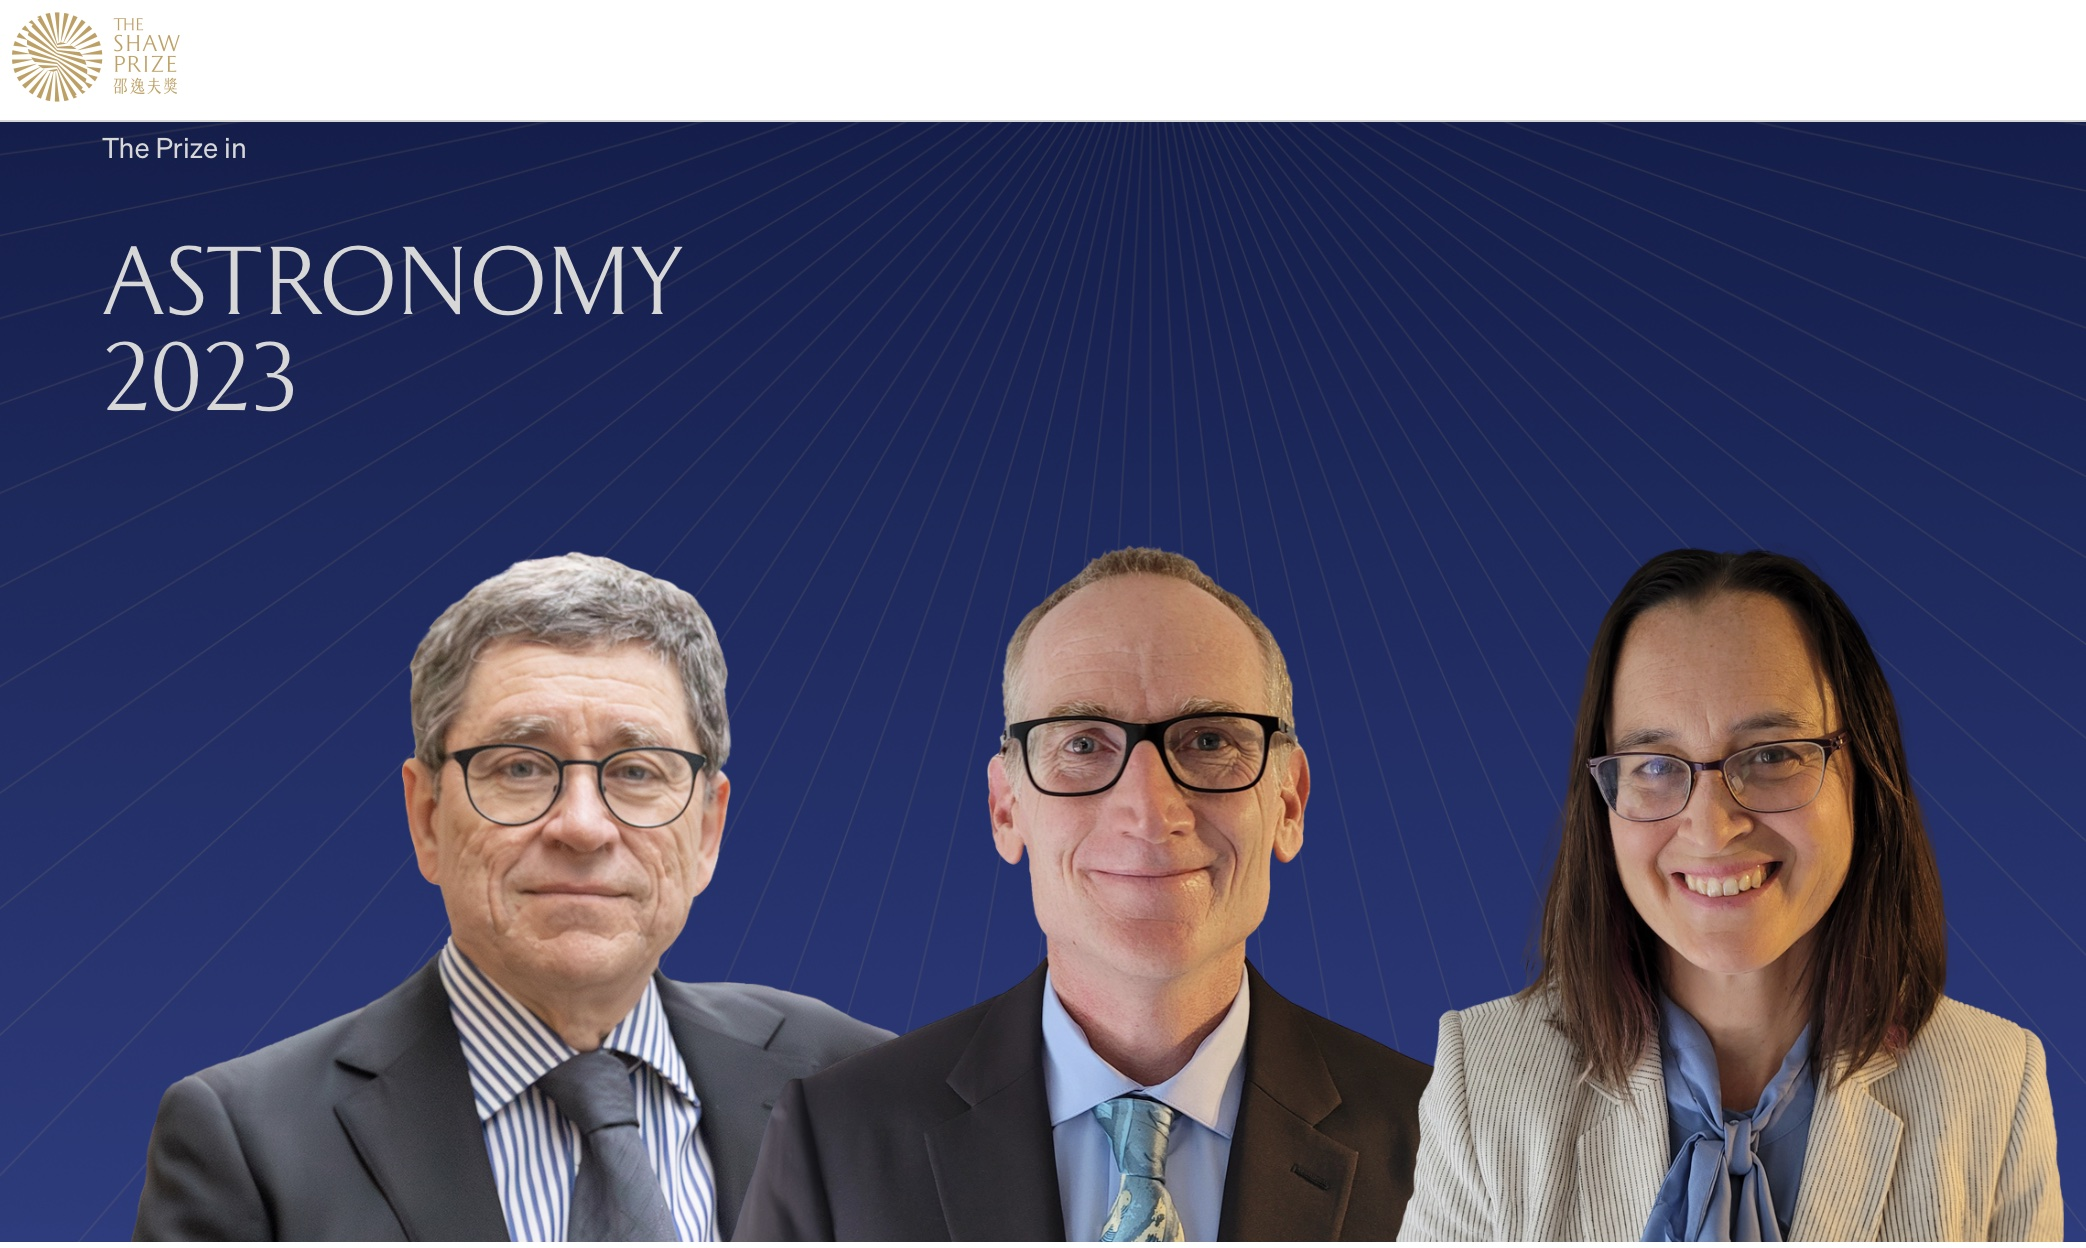
\includegraphics[width=4.5in]{Figures/shaw2023.jpg}
  }


  \frame{
    \frametitle{Fast Radio Bursts}
\small

The Shaw Prize in Astronomy 2023 is awarded in equal shares to {\bf Matthew
Bailes, Duncan Lorimer}, and {\bf Maura McLaughlin} the discovery of fast
radio bursts (FRBs).

FRBs are among the most extreme and mysterious phenomena in astronomy:
they are intense bursts of radio emission lasting only a few
thousandths of a second that contain as much energy as the Sun emits
over several days. The sources of the bursts are smaller than the
Earth but are as far away as distant galaxies. In a seminal research
paper written in 2007, Bailes, Lorimer, McLaughlin (with collaborators
Narkevic and Crawford) found the first FRB; deduced many of the
properties of its source, in particular its extreme distance, small
size, and enormous energy; estimated the cosmic rate of production of
FRBs; and highlighted their potential as cosmological probes.

  }


  \frame{
\vspace{-0.25in}
    \frametitle{FRB110523}
 

%\hspace{2.5in}
\includegraphics[width=2.5in]{Figures/scint110523.png}
\includegraphics[width=1.75in]{Figures/corr110523.png}

Masui++ 2015, Nature, 528, 523
  }



  \frame{
    \frametitle{Fast Radio Bursts}
    \begin{itemize}
        \item Interference effects under multi-path propagation
        \item potential for diffraction limited measurements
        \item Kirchoff-Fresnel path integral
        \item evanescent images
        \item BURSTT
    \end{itemize}
  }

  \frame{
    \frametitle{FRBs}
    \begin{itemize}
      \item thousands detected
      \item increasing sample of well-localized FRBs
        \item Coherent, distant source of radiation
        \item Scintillate under multi-path propagation          
        \item sensitive to ns time delay propagating for gigaparsecs
        \item corresponds to strain $h \ll 10^{-26}$: far exceeds LIGO
        \item highly elongated antenna pattern: sensitive to
          longitudinal modes          
    \end{itemize}
  }

  \frame{
    \frametitle{What are they?}
    \begin{itemize}
      \item mean luminosity: modest ($\lesssim 10^{40}$ erg/s)
      \item instantaneous intensity: $\sim 10^{40}$K
        \item beaming?
        \item pulsar analogs: crab beaming, companion plasma lensing,
          etc.  
          \item measured $\gamma \sim 10^4$, beaming correction $\sim 10^8$
        \item not seen in MW. Rare event, Short life span?
    \end{itemize}
  }


  \frame{

    \frametitle{TDE recyling?}
\begin{center}
\includegraphics[width=2.1in]{Figures/lipen.jpg}
\end{center}
  }
  \frame{

    \frametitle{PSR B0834+06: Coherent VLBI}
\vspace{-0.25in}
\begin{center}
\hspace{-0.5in}
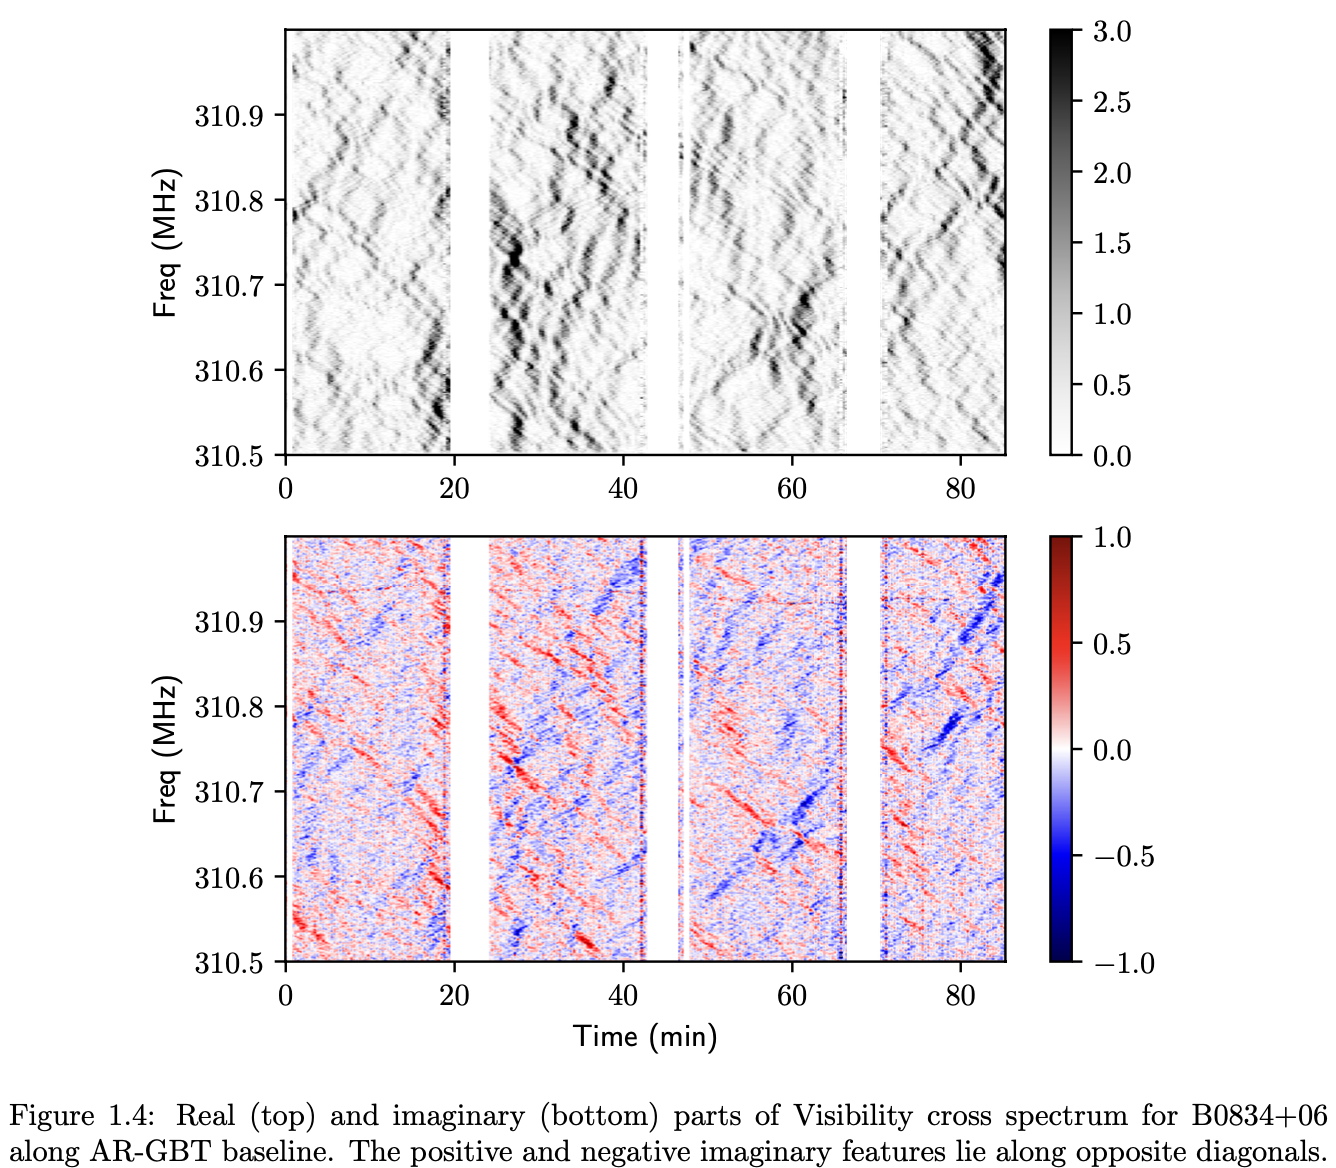
\includegraphics[width=3.5in]{Figures/rawvlbi.png}
\end{center}
  }
  \frame{
%\vspace{-0.25in}
    \frametitle{Scintillometry VLBI}
\hspace{-0.25in}
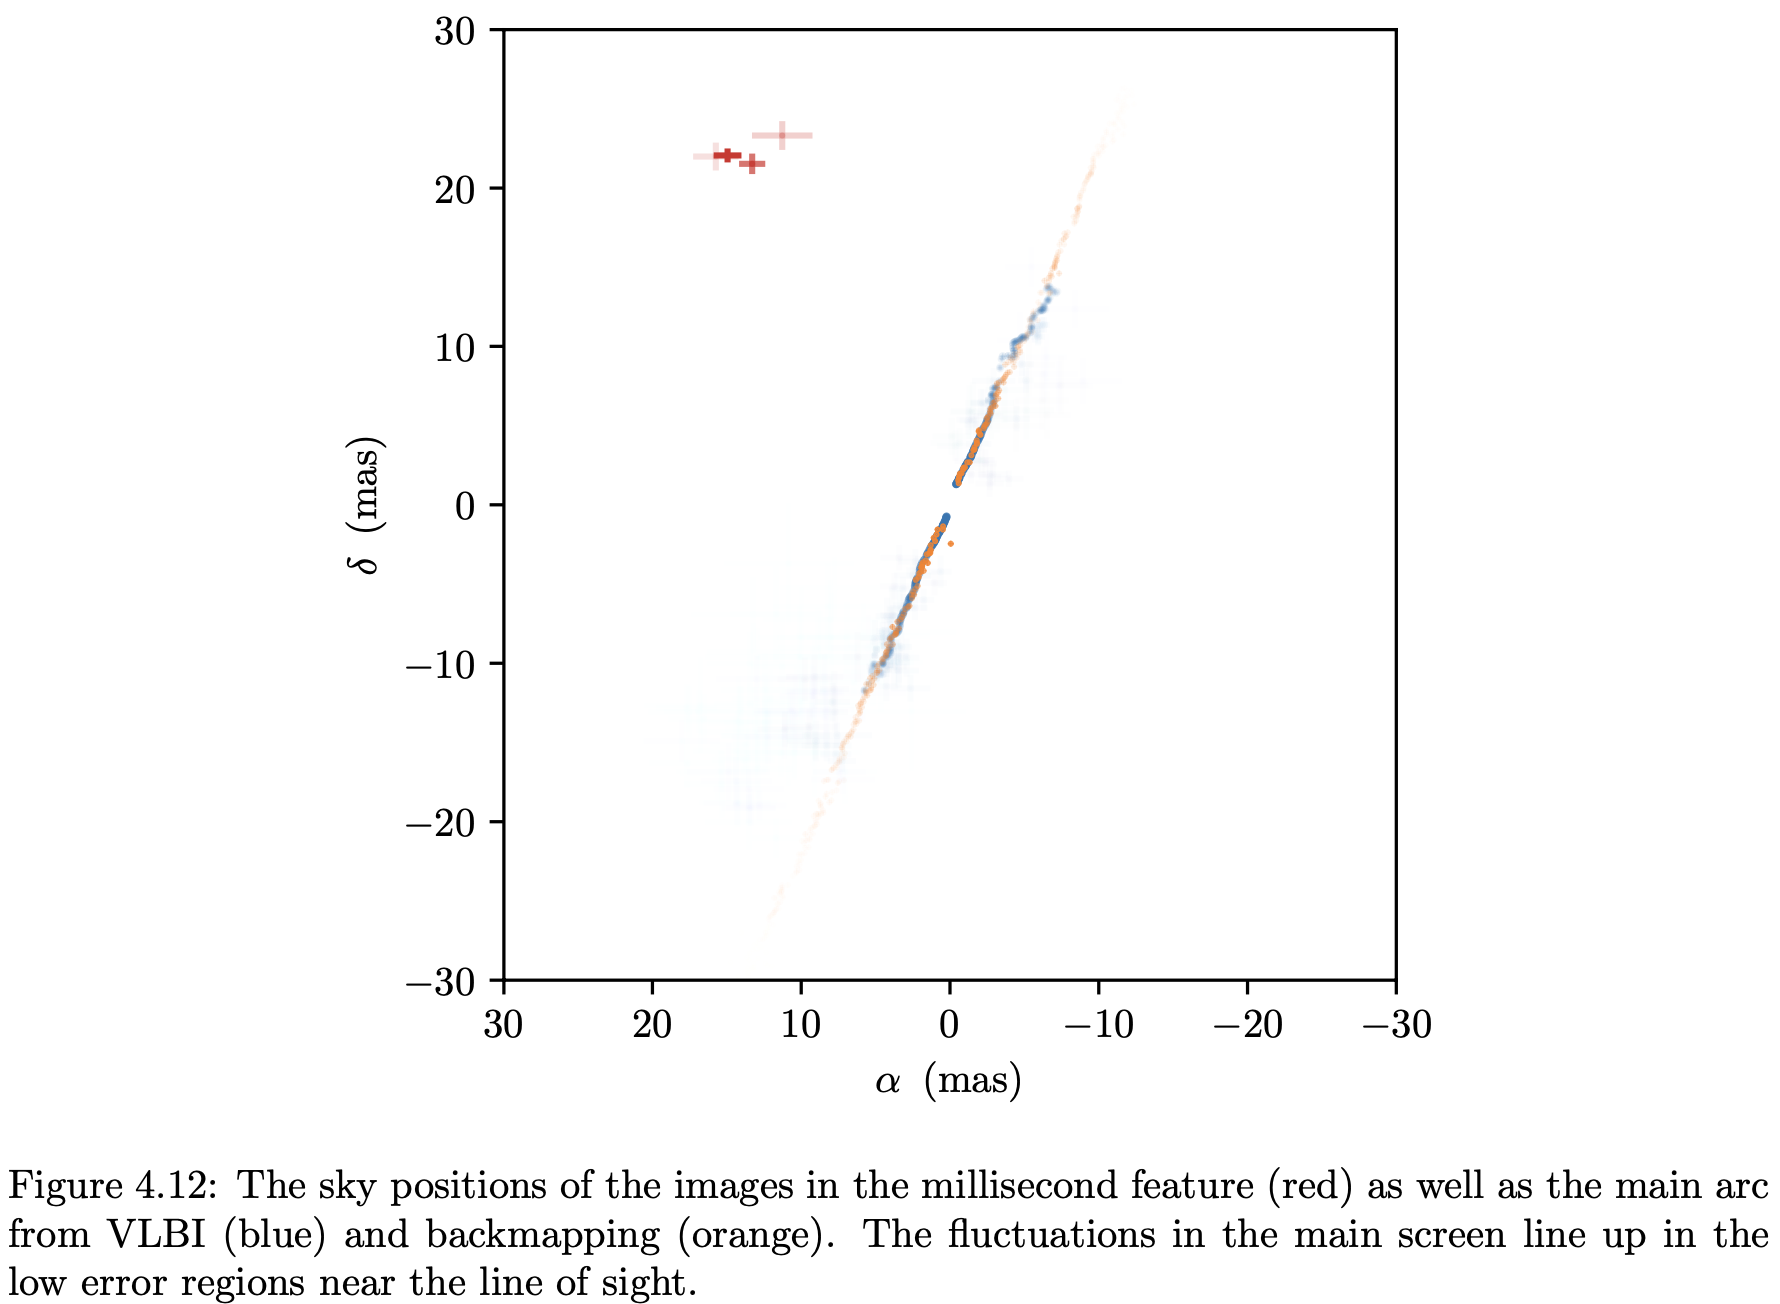
\includegraphics[width=3.5in]{Figures/VLBI0834.png}
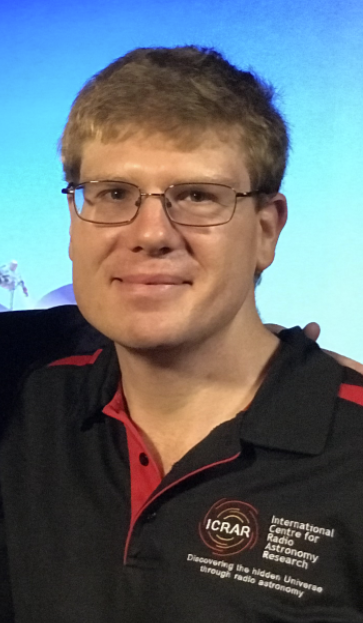
\includegraphics[width=1.05in]{Figures/jpm.png}

Baker++: increase PTA angular resolution to arcminutes.  In memoriam J-P Macquart.
  }


  \frame{

    \frametitle{precision astrometry}
\vspace{-0.25in}
\begin{center}
\hspace{-0.5in}
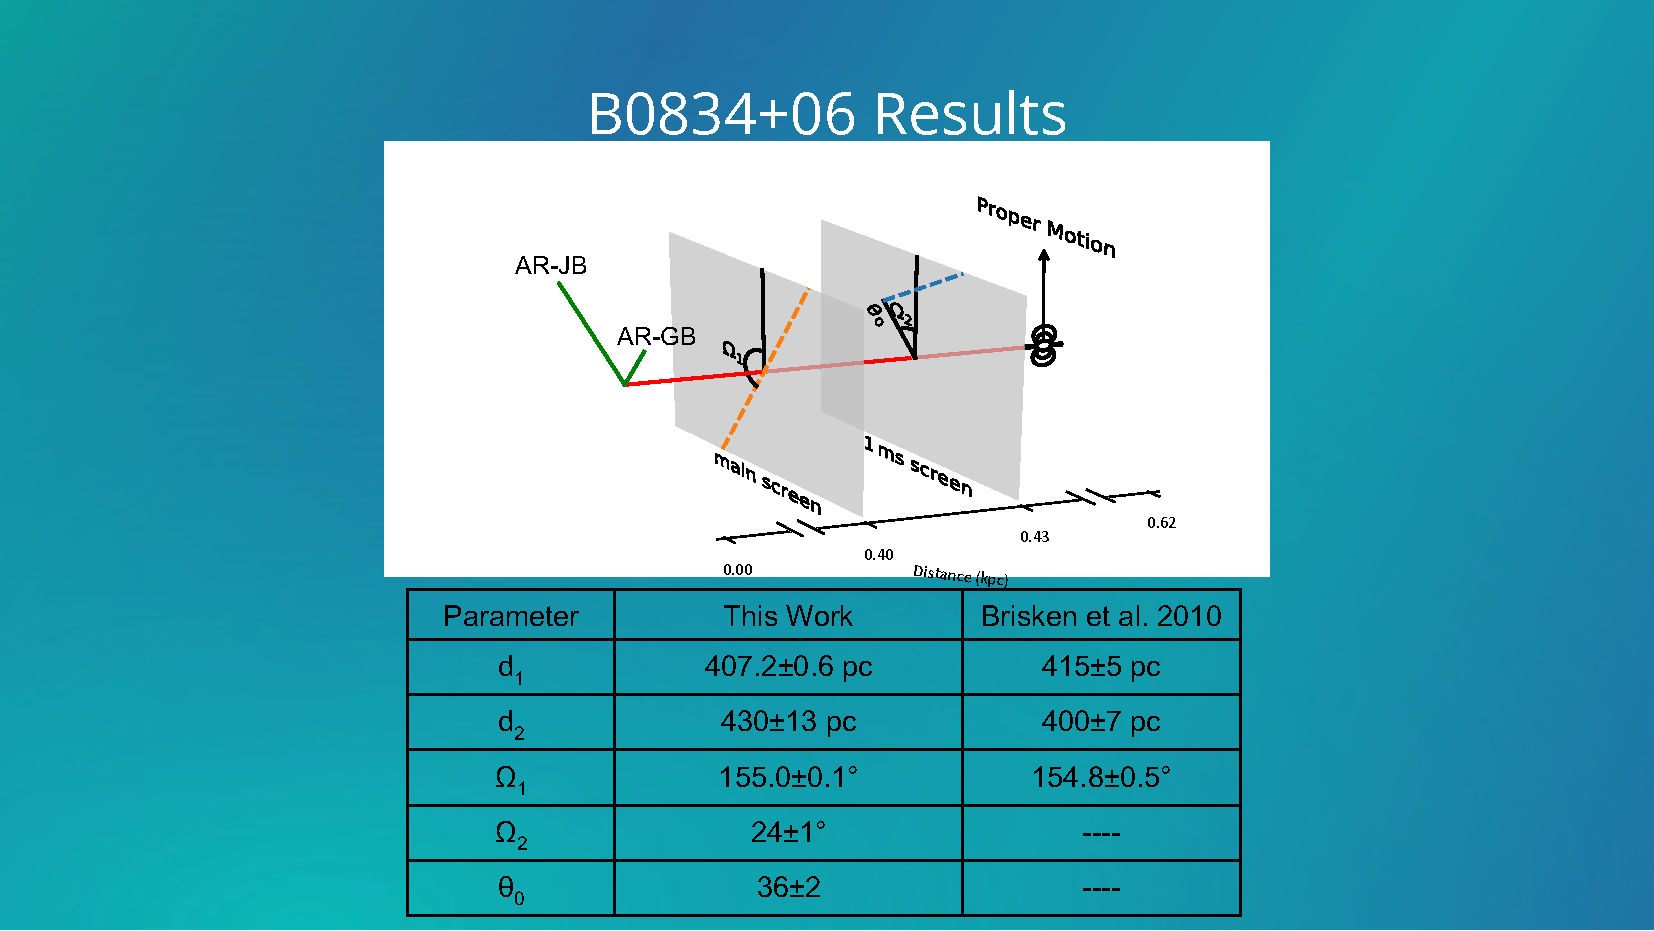
\includegraphics[width=5.5in]{Figures/VLBIdist.pdf}
\end{center}
  }


  \frame{

    \frametitle{more precision astrometry}
%\vspace{-0.25in}
\begin{center}
%\hspace{-0.5in}
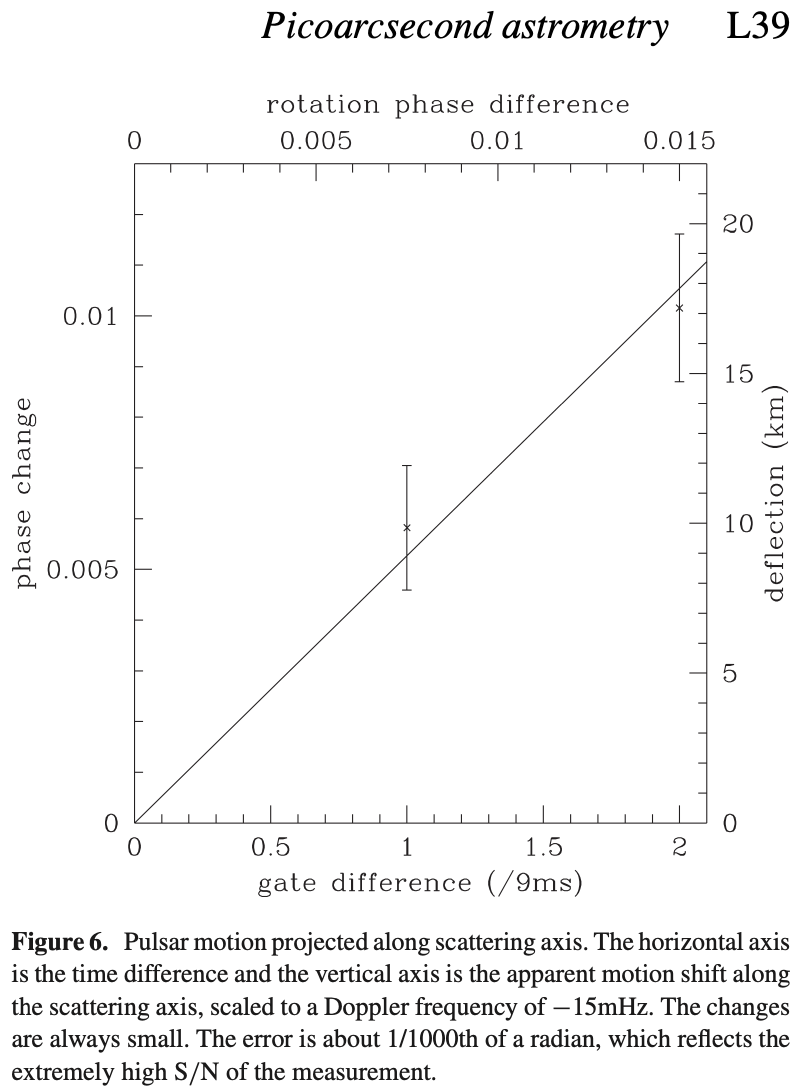
\includegraphics[width=2.05in]{Figures/pico.png}
UP+14
\end{center}
  }


  \frame{
\vspace{-0.25in}
    \frametitle{Optics: Geometric, Eikonal, Wave, P-L}
    \begin{itemize}
        \item Consider 1-D lens
        \item lensing potential $\Psi(\theta)$
        \item deflection $\Psi'$
        \item simplify for $D_{\rm ds}=\infty$
    \end{itemize}
\vspace{-0.5in}\hspace{2.5in}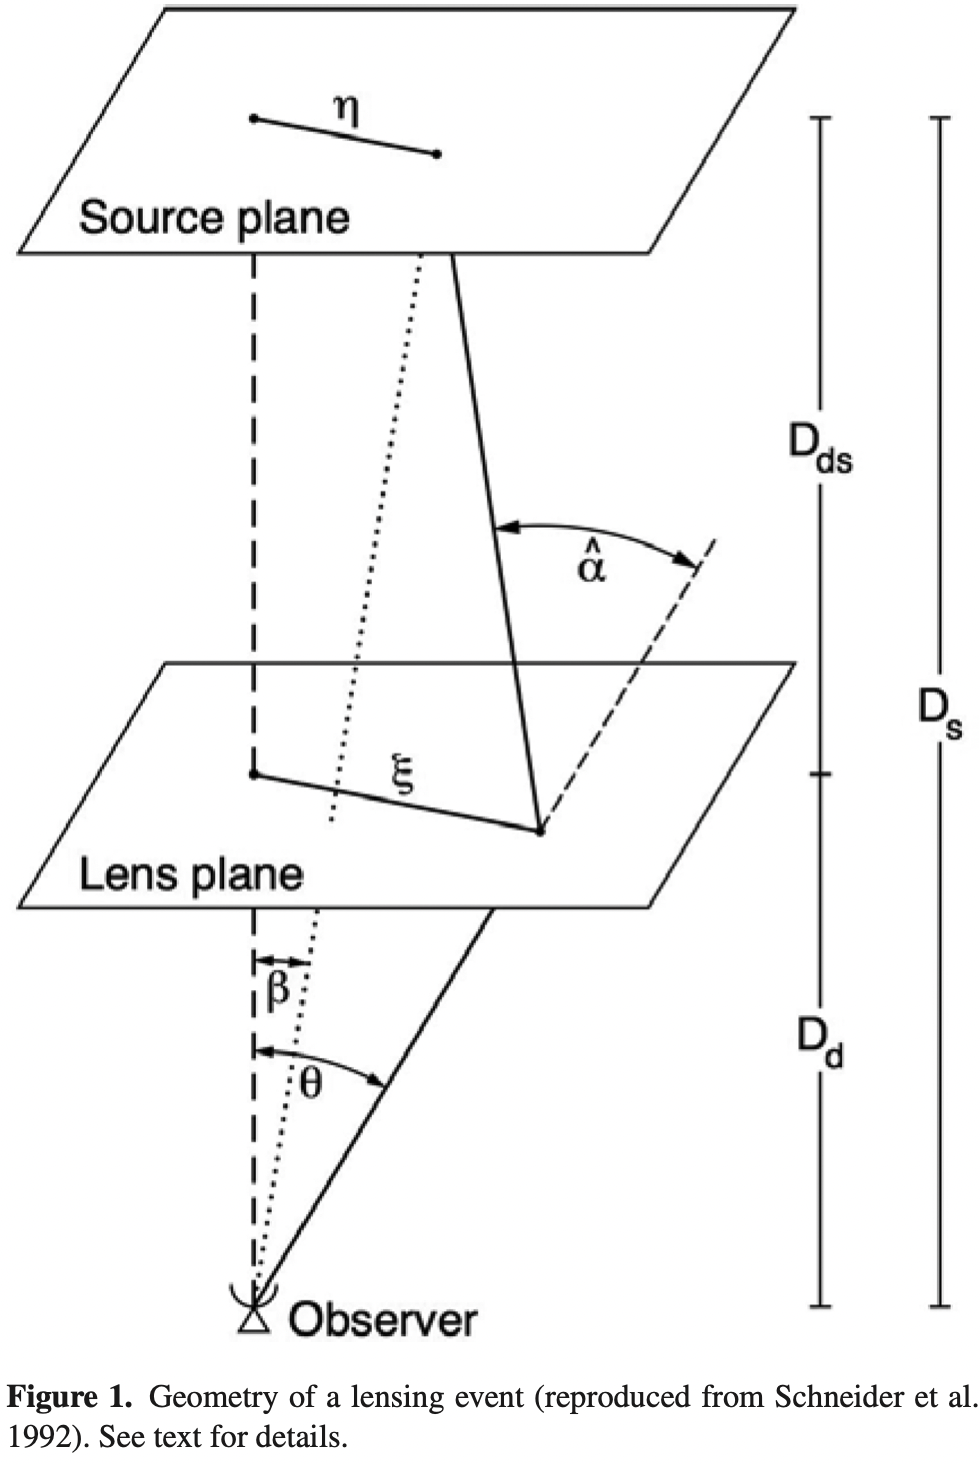
\includegraphics[width=1.5in]{Figures/lens.png}

  }


  \frame{
\vspace{-0.25in}
    \frametitle{Huygen's Principle: Path Integral}
    \begin{itemize}
        \item $A(\mu)=\int e^{i S(\theta,\mu)} d\theta$ 
        \item $S=\nu [(\theta-\mu)^2+\Psi(\theta)]$
        \item Highly oscillatory integral, even for $\Psi=0$
        \item Stationary phase points: $\partial_\theta S=0$ leads to (complex)
          Eikonal images $\theta_i$.
        \item flux/phase through curvature expansion (known as {\it
            steepest descent}): exact as $\nu \rightarrow \infty$
        \item Geometric limit considers only {\it Real} solutions $\theta_i$ and
      gives up phase
          information (length of trajectory)
        \item Geometric optics applicable at short wavelengths for
          extended sources
          (e.g. optical gravitational lensing of finite size sources,
          stars)     
          \item roughly 1/4 of the degrees of freedom of Eikonal 
    \end{itemize}
  }
  \frame{
\vspace{-0.5in}
    \frametitle{Evanescent Images}
    \begin{itemize}
    \item consider ``rational lens'' potential $\psi(\theta)=\alpha/(1+\theta^2)$
    \item Geometric/eikonal images at $\psi'=\theta$
    \item 5 roots.  1 or 3 real roots, rest imaginary
    \item P-L: at most one imaginary image contributes!
    \item Resurgence theory to classify?
    \item Evanescent (imaginary) image can be brighter than unlensed real image
    \end{itemize}
  }


  \frame{
%\vspace{-0.5in}
    \frametitle{Rational 1-D lens}
\begin{center}
\includegraphics[width=3.1in]{Figures/theta-beta.eps}
\end{center}
  }

  
  \frame{
\vspace{-0.5in}
    \frametitle{Picard-Lefschetz Theory}
    \begin{itemize}
    \item descend integral along real line along Morse function Im(S)
    \item contour deforms into finite number of Thimbles of constant
      phase with maximum at saddle point (extrema $dS=0$)
    \item correctly identifies relevant saddle points
    \item resolves numerical challenges of oscillatory integral
    \item complex analysis works in multiple variables
    \item elevates concept of ``image'' deep into wave optics
    \item multiple public implementations (Feldbrugge+, Jow+)
    \end{itemize}
  }




  \frame{
\vspace{-0.5in}
    \frametitle{Picard-Lefschetz Theory}

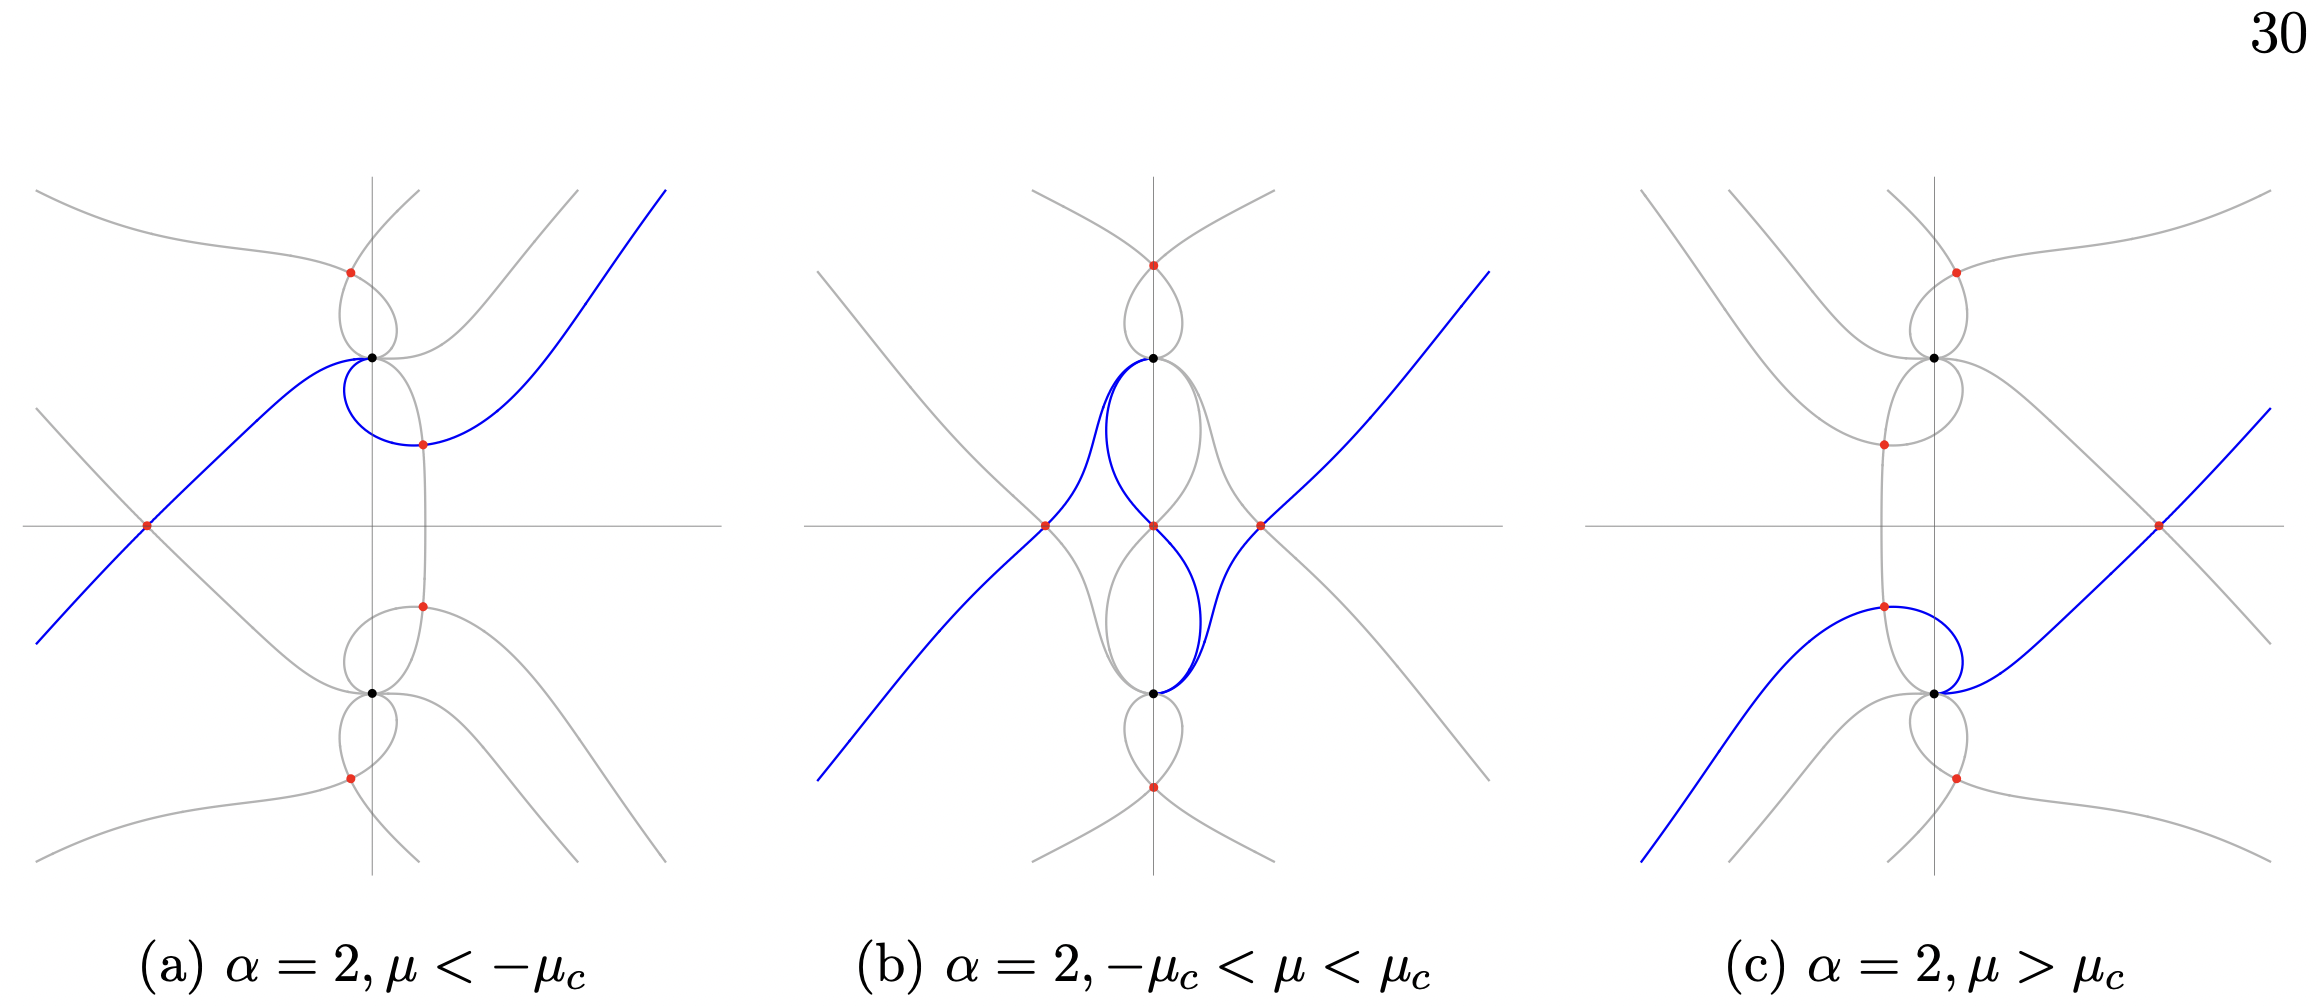
\includegraphics[width=4.5in]{Figures/thimbles.png}

Feldbrugge+2019
  }


  

  \frame{
\vspace{-0.5in}
    \frametitle{New Observables}
    \begin{itemize}
    \item for coherent sources: FRBs, pulsars
    \item weak lensing: imaginary image allows time delay measurement (Jow+21)
    \item strong lensing: delay measurements enable measurement of
      co-linearity (Jow++21)
    \item microlensing: instant time delay, planets (Jow+20)
    \item macrolensing: potentially nano-second delay -- universe
      expands!  Dark energy, etc (Wucknitz+21)
    \item dimensionless strain cm/Gigalightyears $h\sim \Delta t/t \sim 10^{-26}$:
      competitive with LIGO, etc
    \end{itemize}
  }


  \frame{

    \frametitle{Catastrophes}
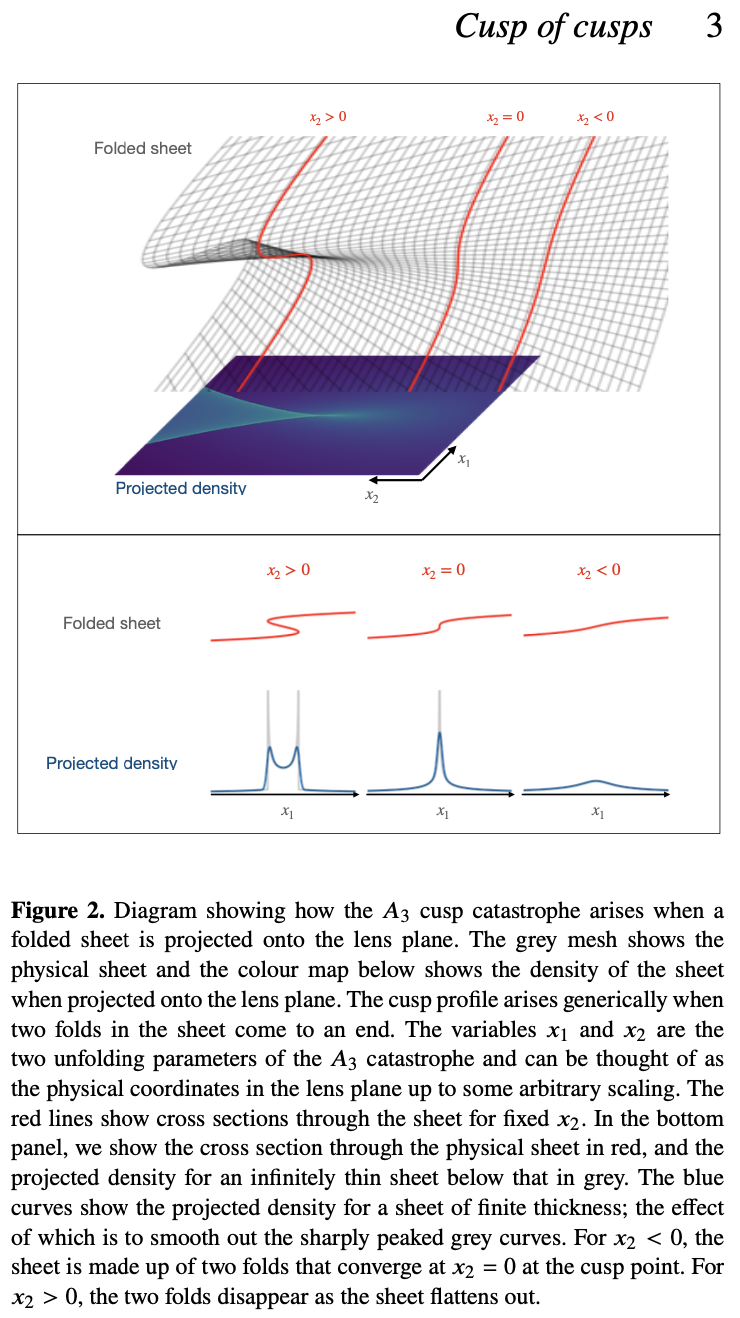
\includegraphics[width=2.85in]{Figures/cusp.png}
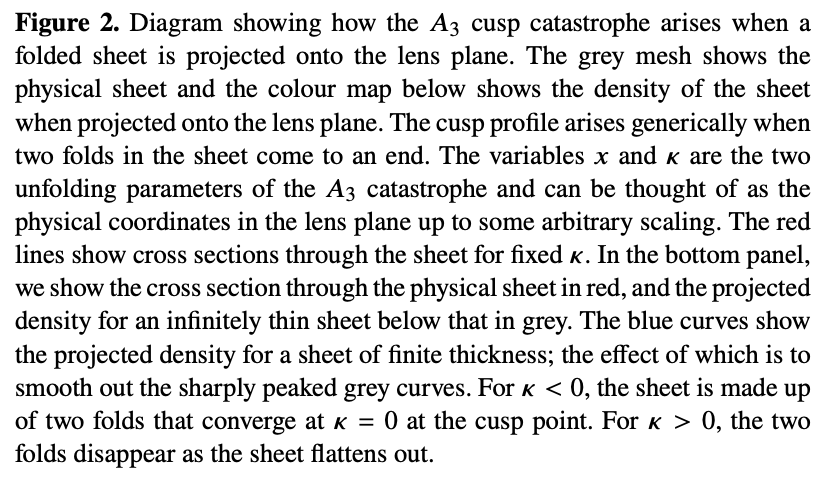
\includegraphics[width=0.5in]{Figures/cuspcaption.png}
Jow+2301.08344
  }

    \frametitle{Extreme Scattering Events}
%\hspace{-0.5in}
\begin{center}
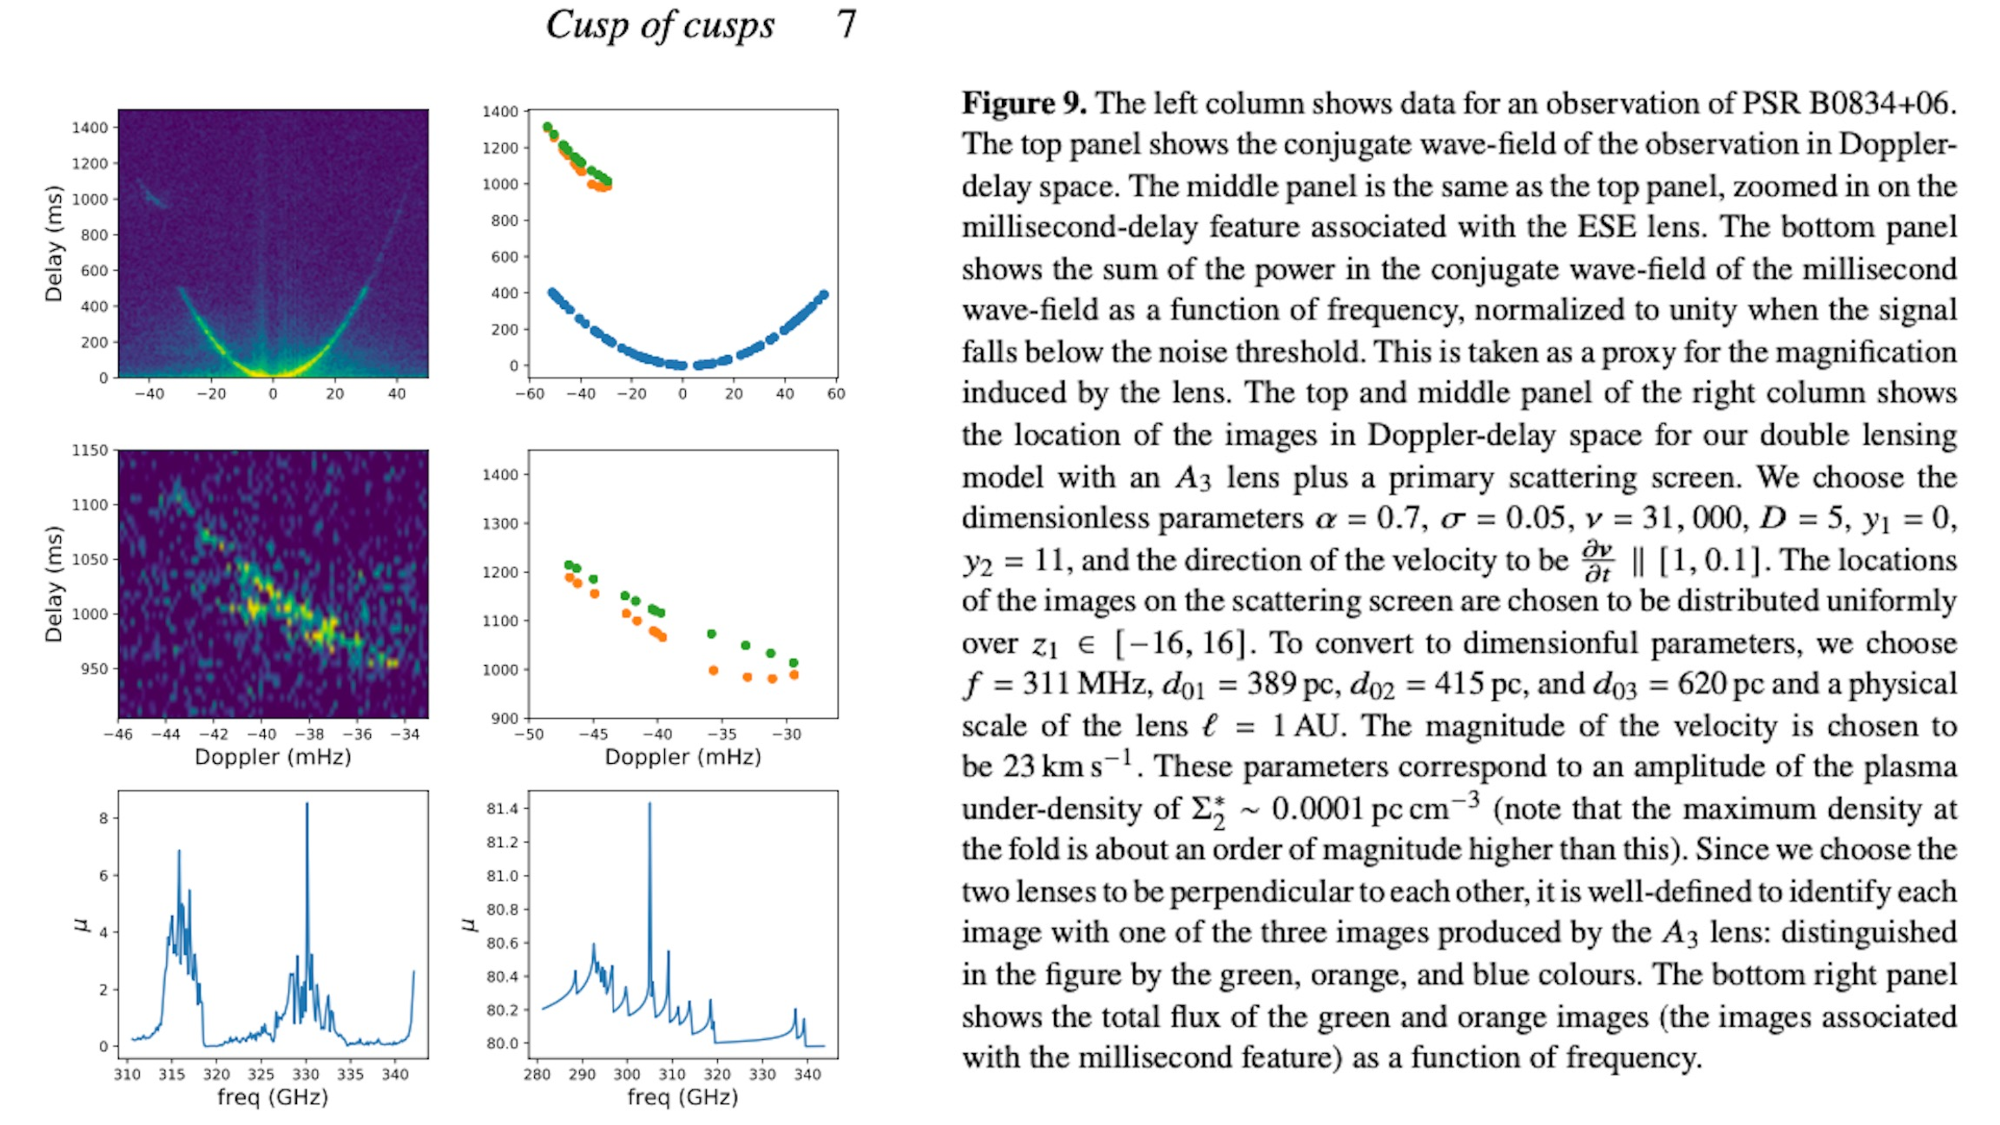
\includegraphics[width=4.65in]{Figures/esemodel.pdf}
\end{center}
  }


  \frame{
%\vspace{-0.25in}
    \frametitle{Macro lensing}
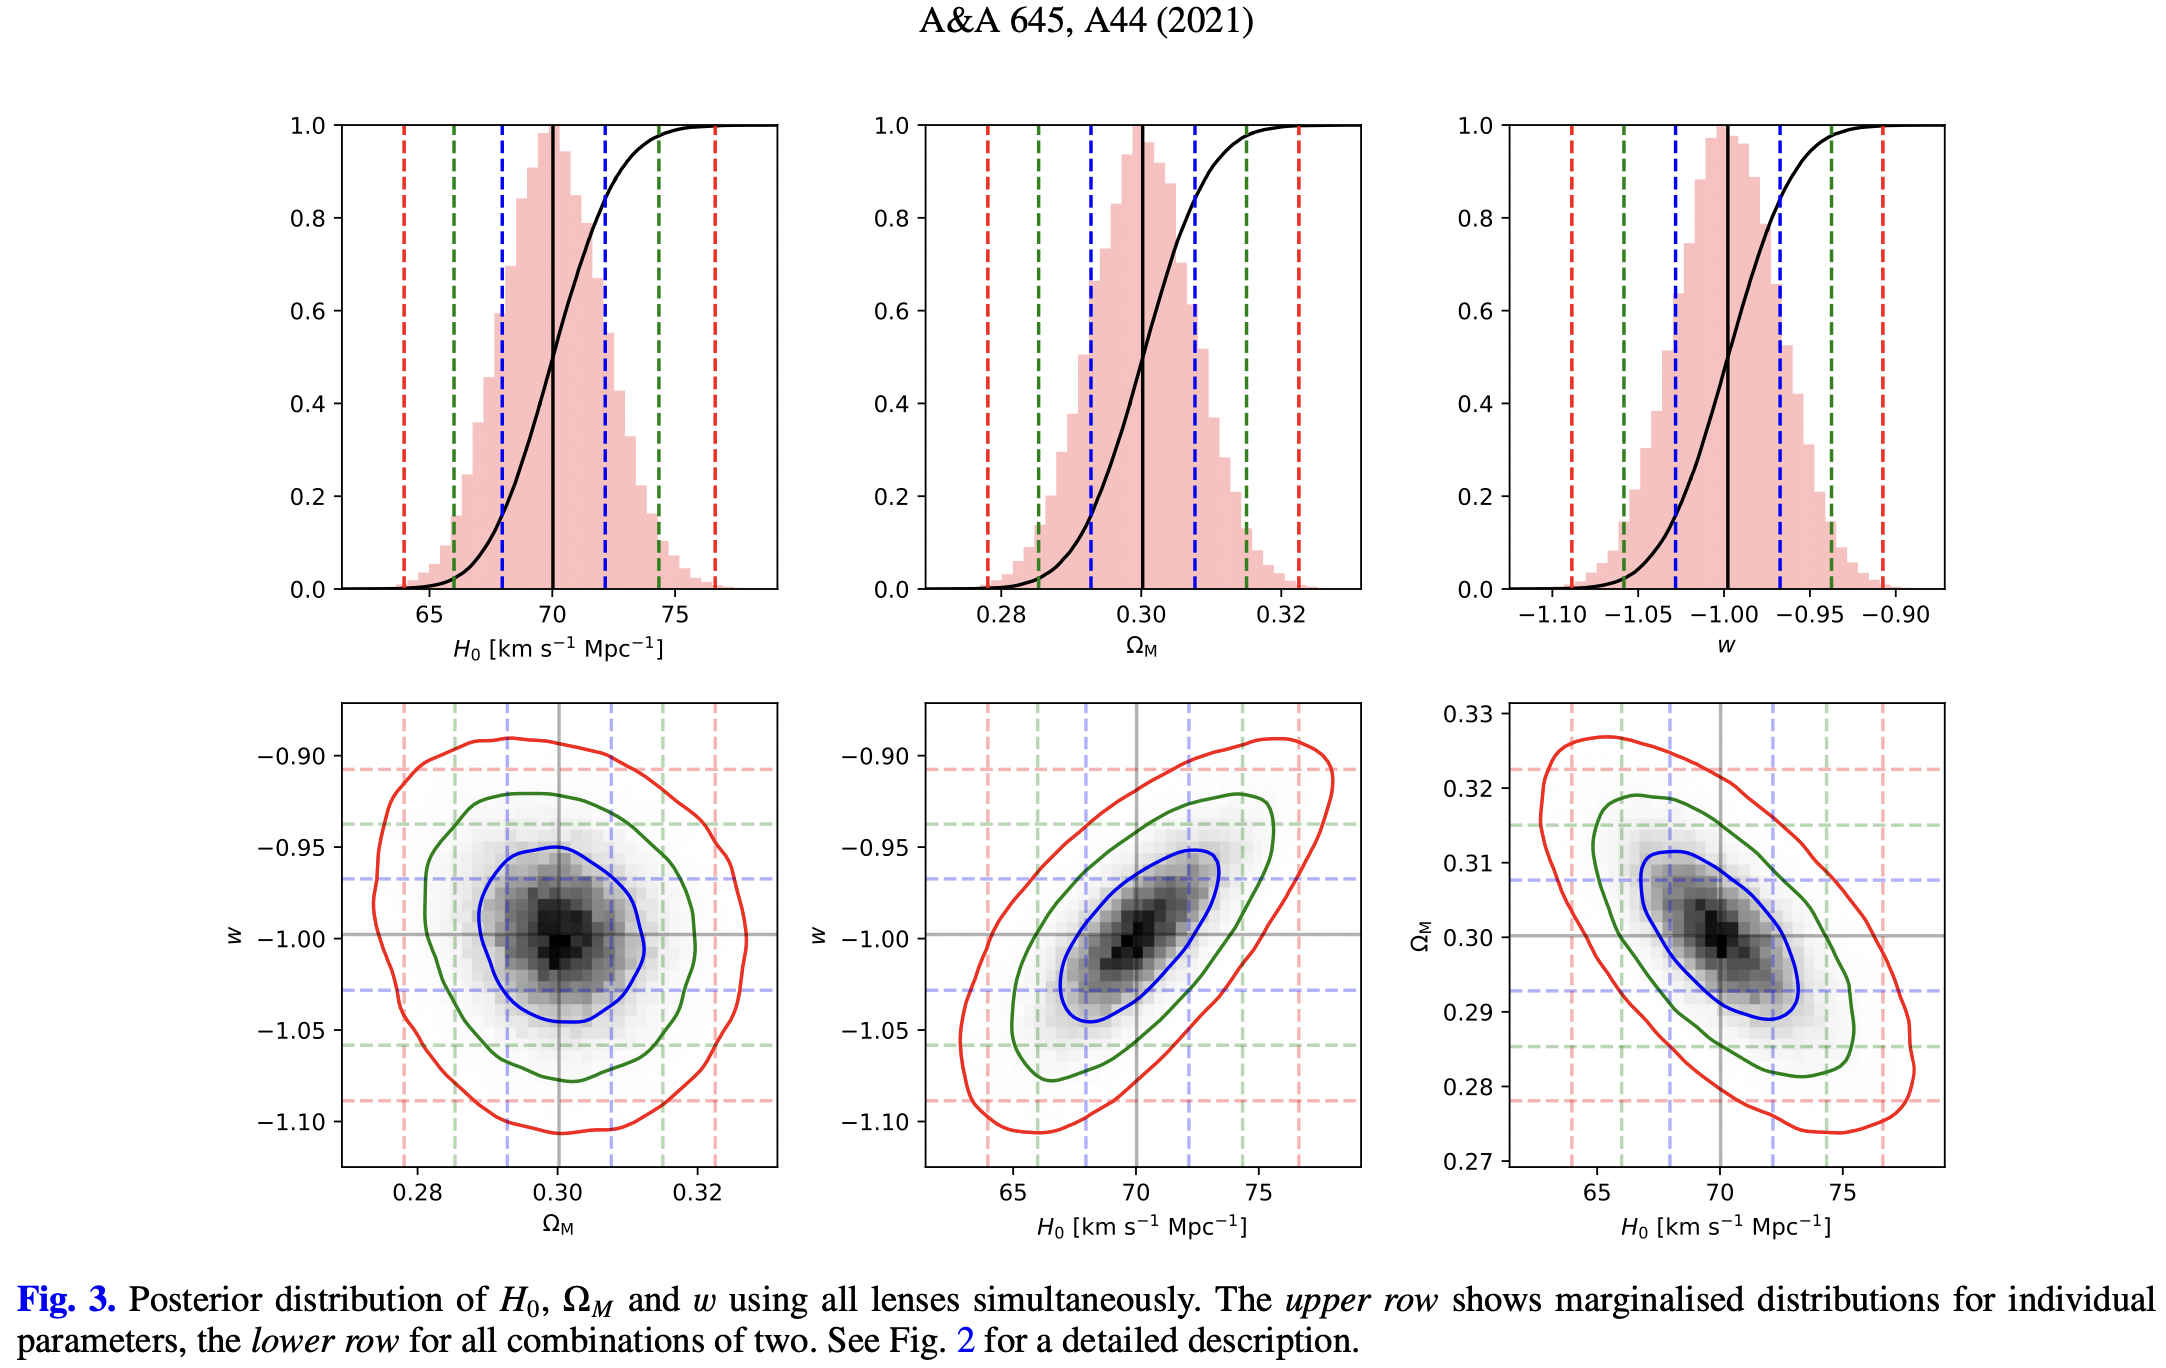
\includegraphics[width=4.5in]{Figures/wucknitz.png}

Wucknitz, Spitler, ULP 2021, A\&A, 645, A44
  }




  \frame{
\vspace{-0.5in}
    \frametitle{Discussion}
    \begin{itemize}
    \item Eikonal effects applicable to compact radio sources,
      e.g. FRBs, pulsars
    \item full wave
effect dominates for long wavelengths as Fresnel scale is bigger then Einstein radius
    \item microlensing down to planet size
    \item gravitational waves:  LIGO, LISA, PTA
    \end{itemize}
  }

  \frame{
\vspace{-0.5in}
    \frametitle{BURSTT}
    \begin{itemize}
    \item Bustling Universe Radio Survey Telescope in Taiwan
    \item instant wide field, VLBI localization
    \item nearby counterparts, multi-wavelength, multi-messenger
    \item repeat statistics
    \item bright sample for deep followup
    \end{itemize}
  }


  \frame{
    \frametitle{BURSTT}
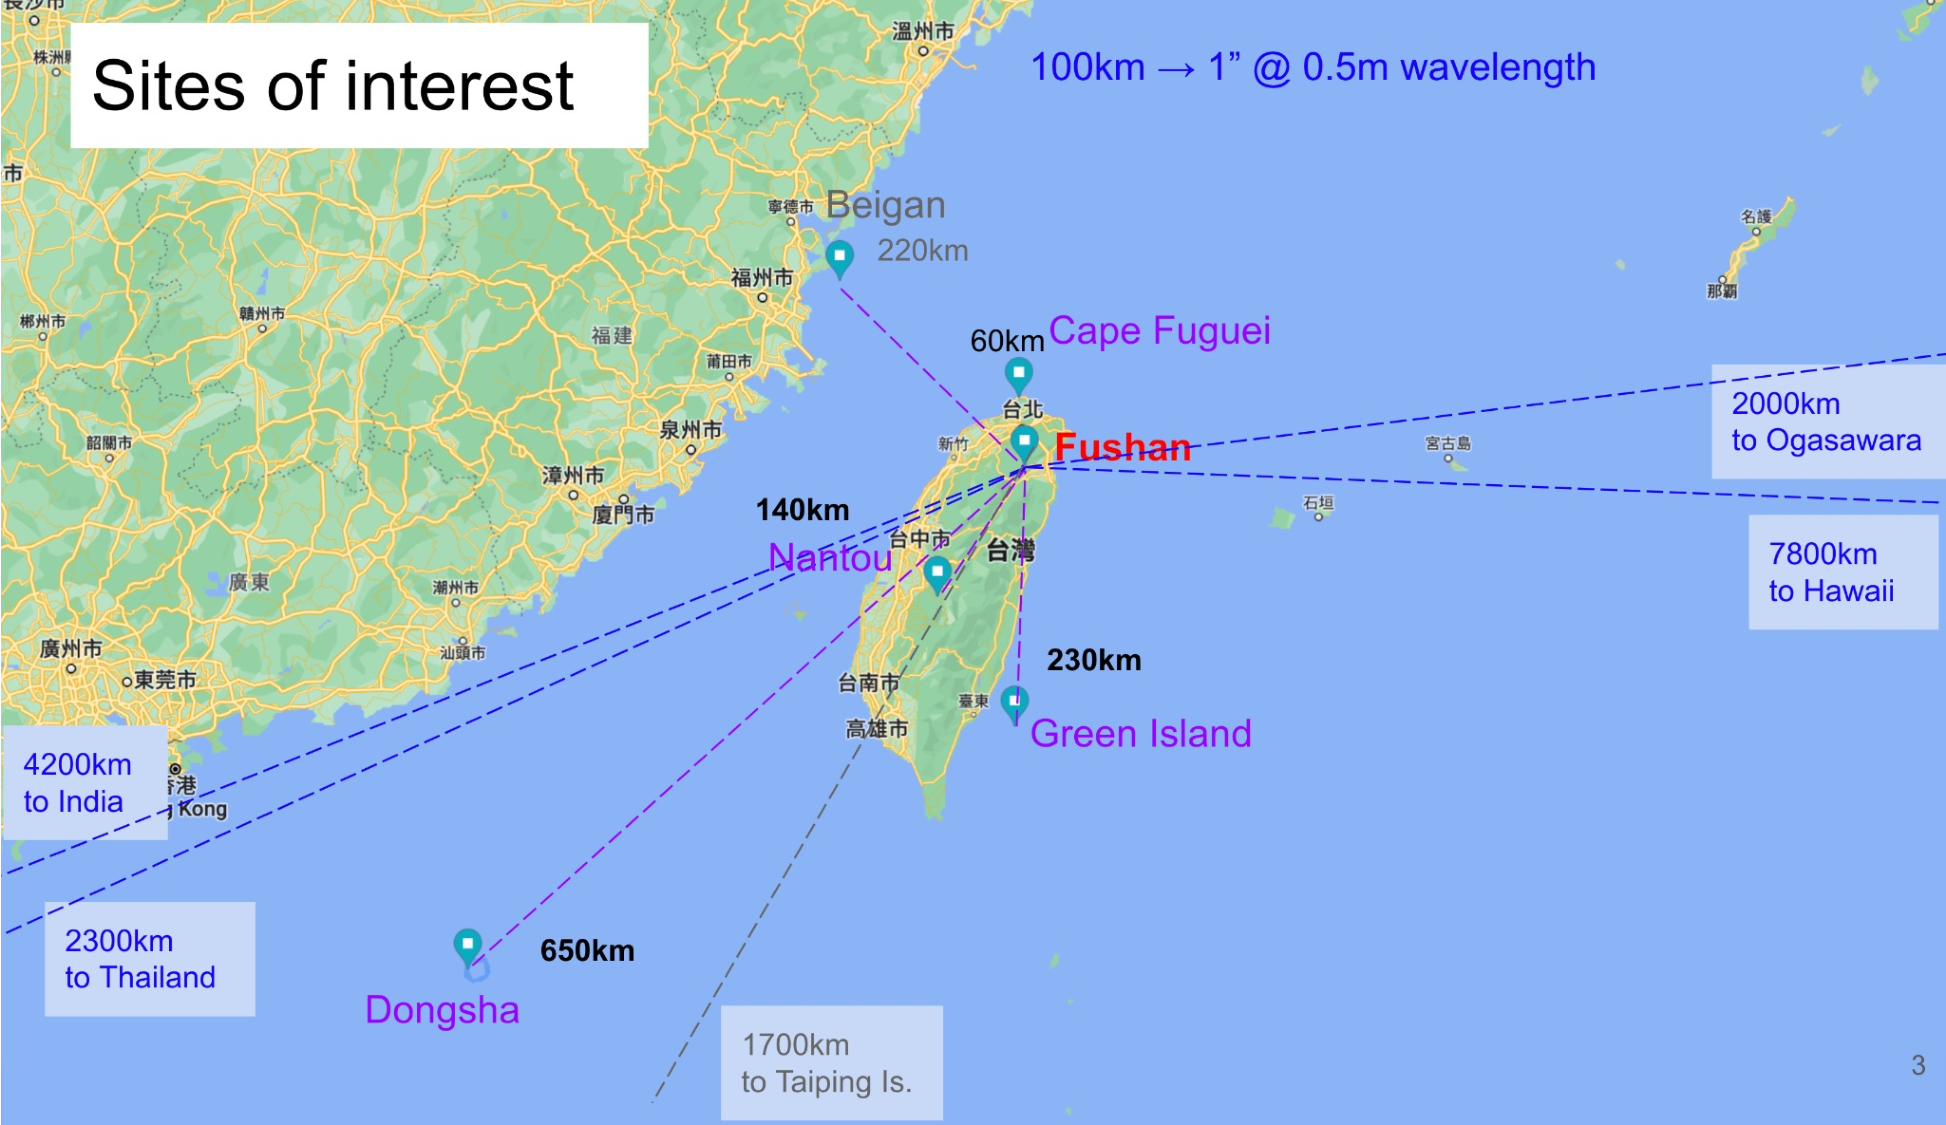
\includegraphics[width=4.5in]{Figures/bursttsites.pdf}
  }


  \frame{
    \frametitle{Fushan}
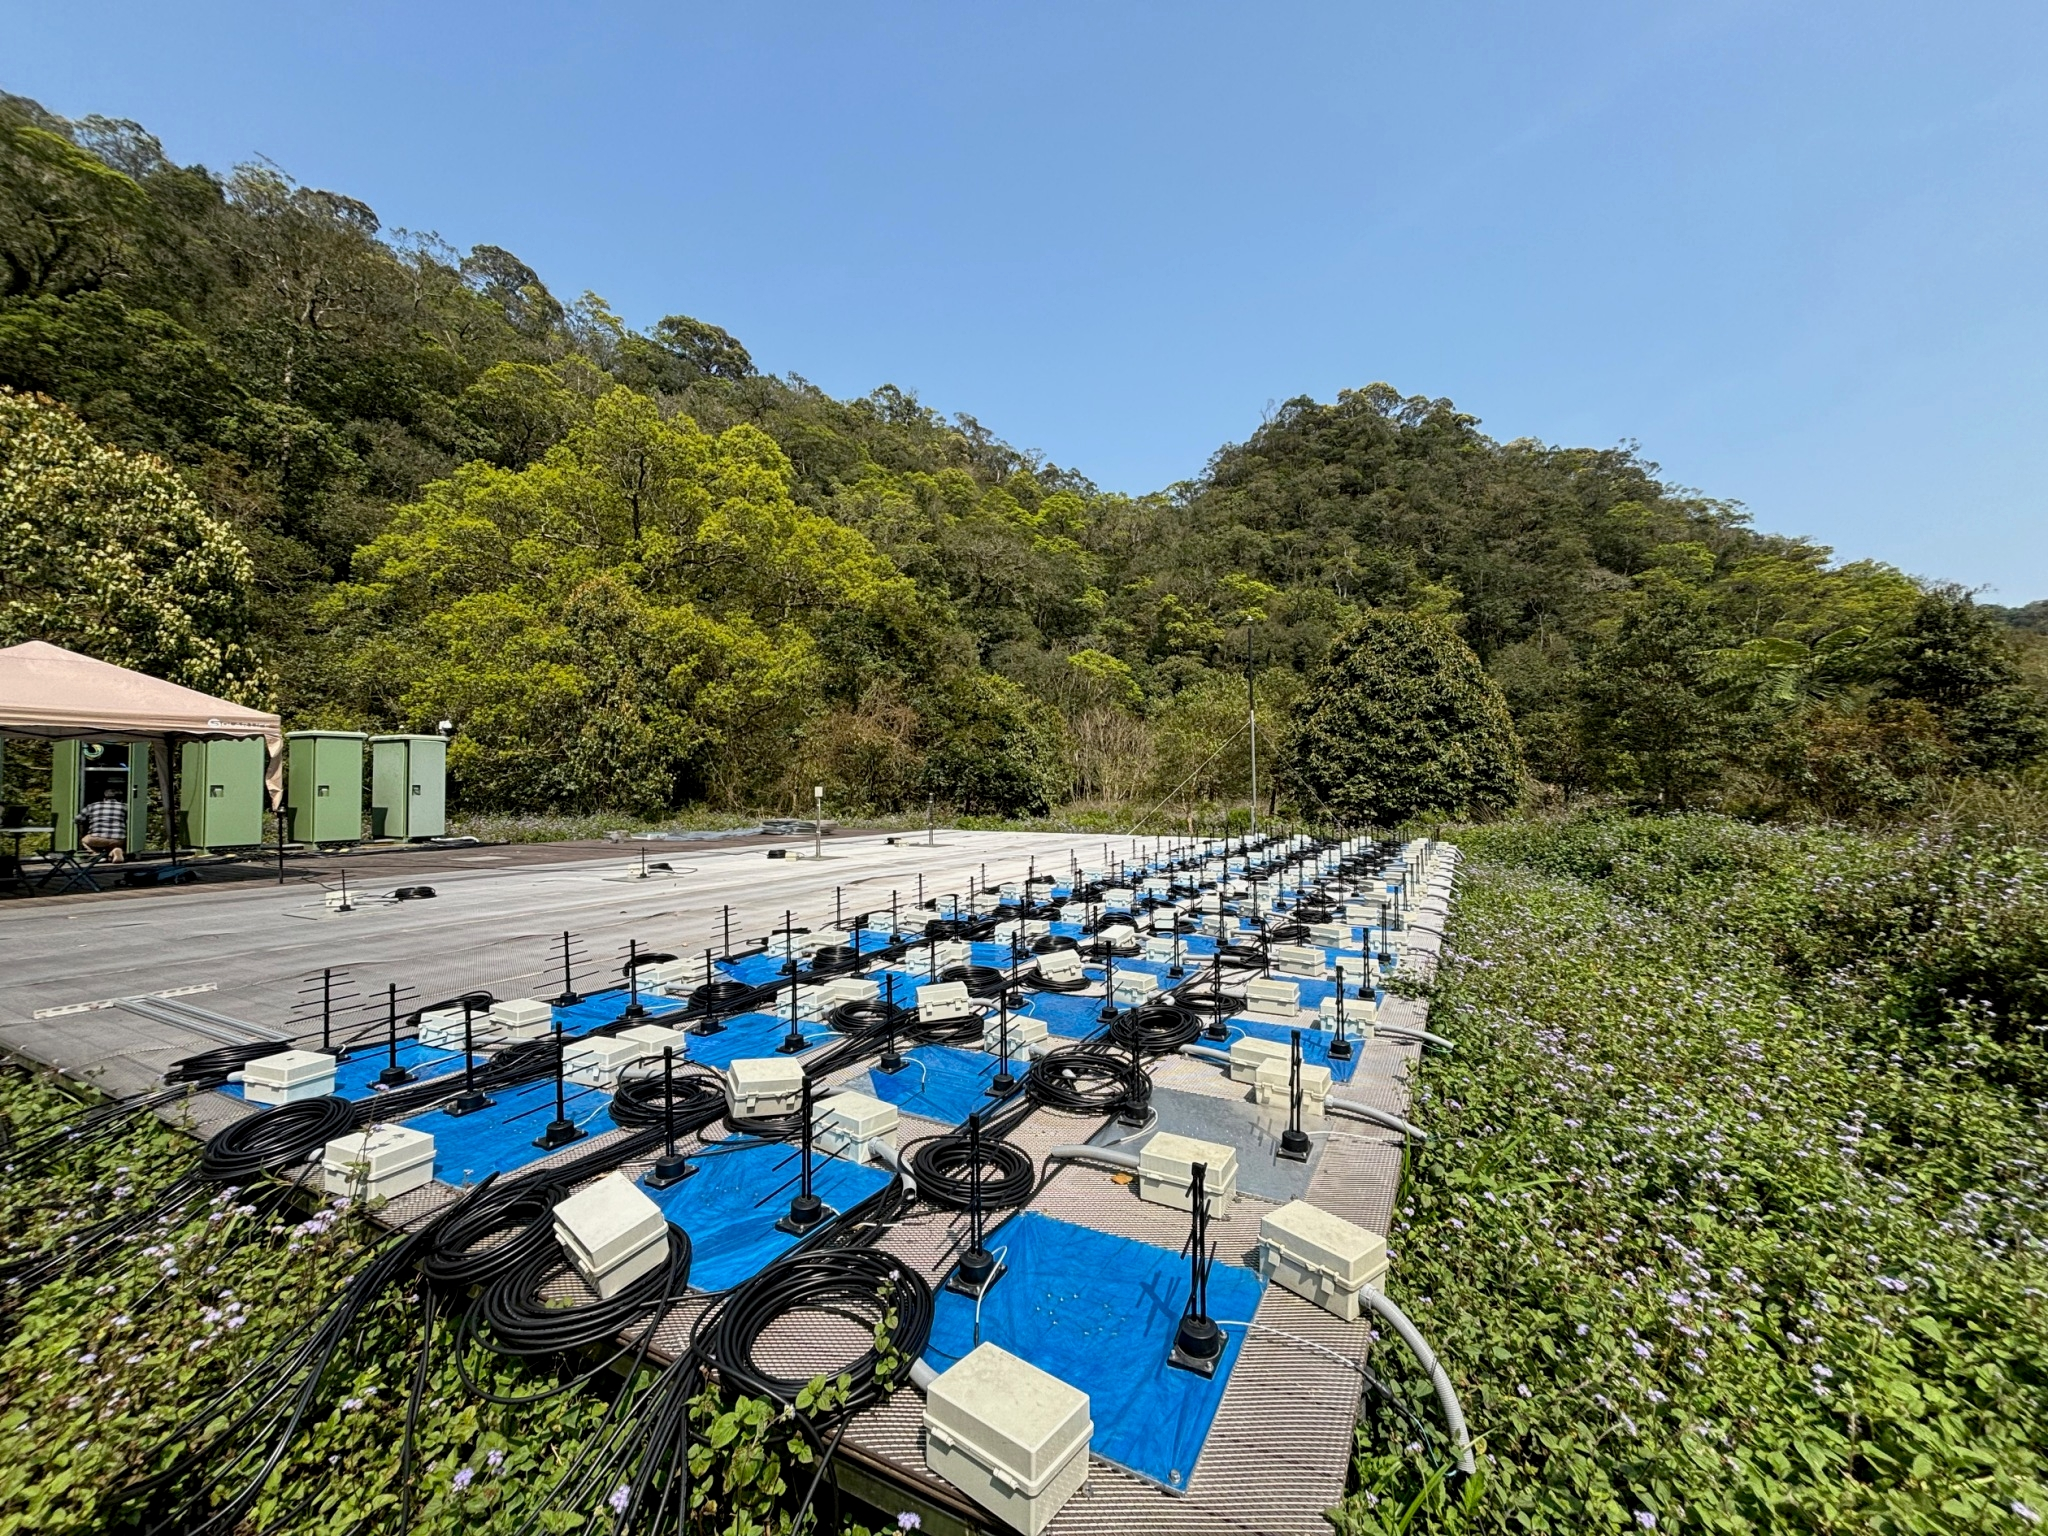
\includegraphics[width=4.5in]{Figures/fushan2024.jpg}
  }

  \frame{
    \frametitle{Nantou}
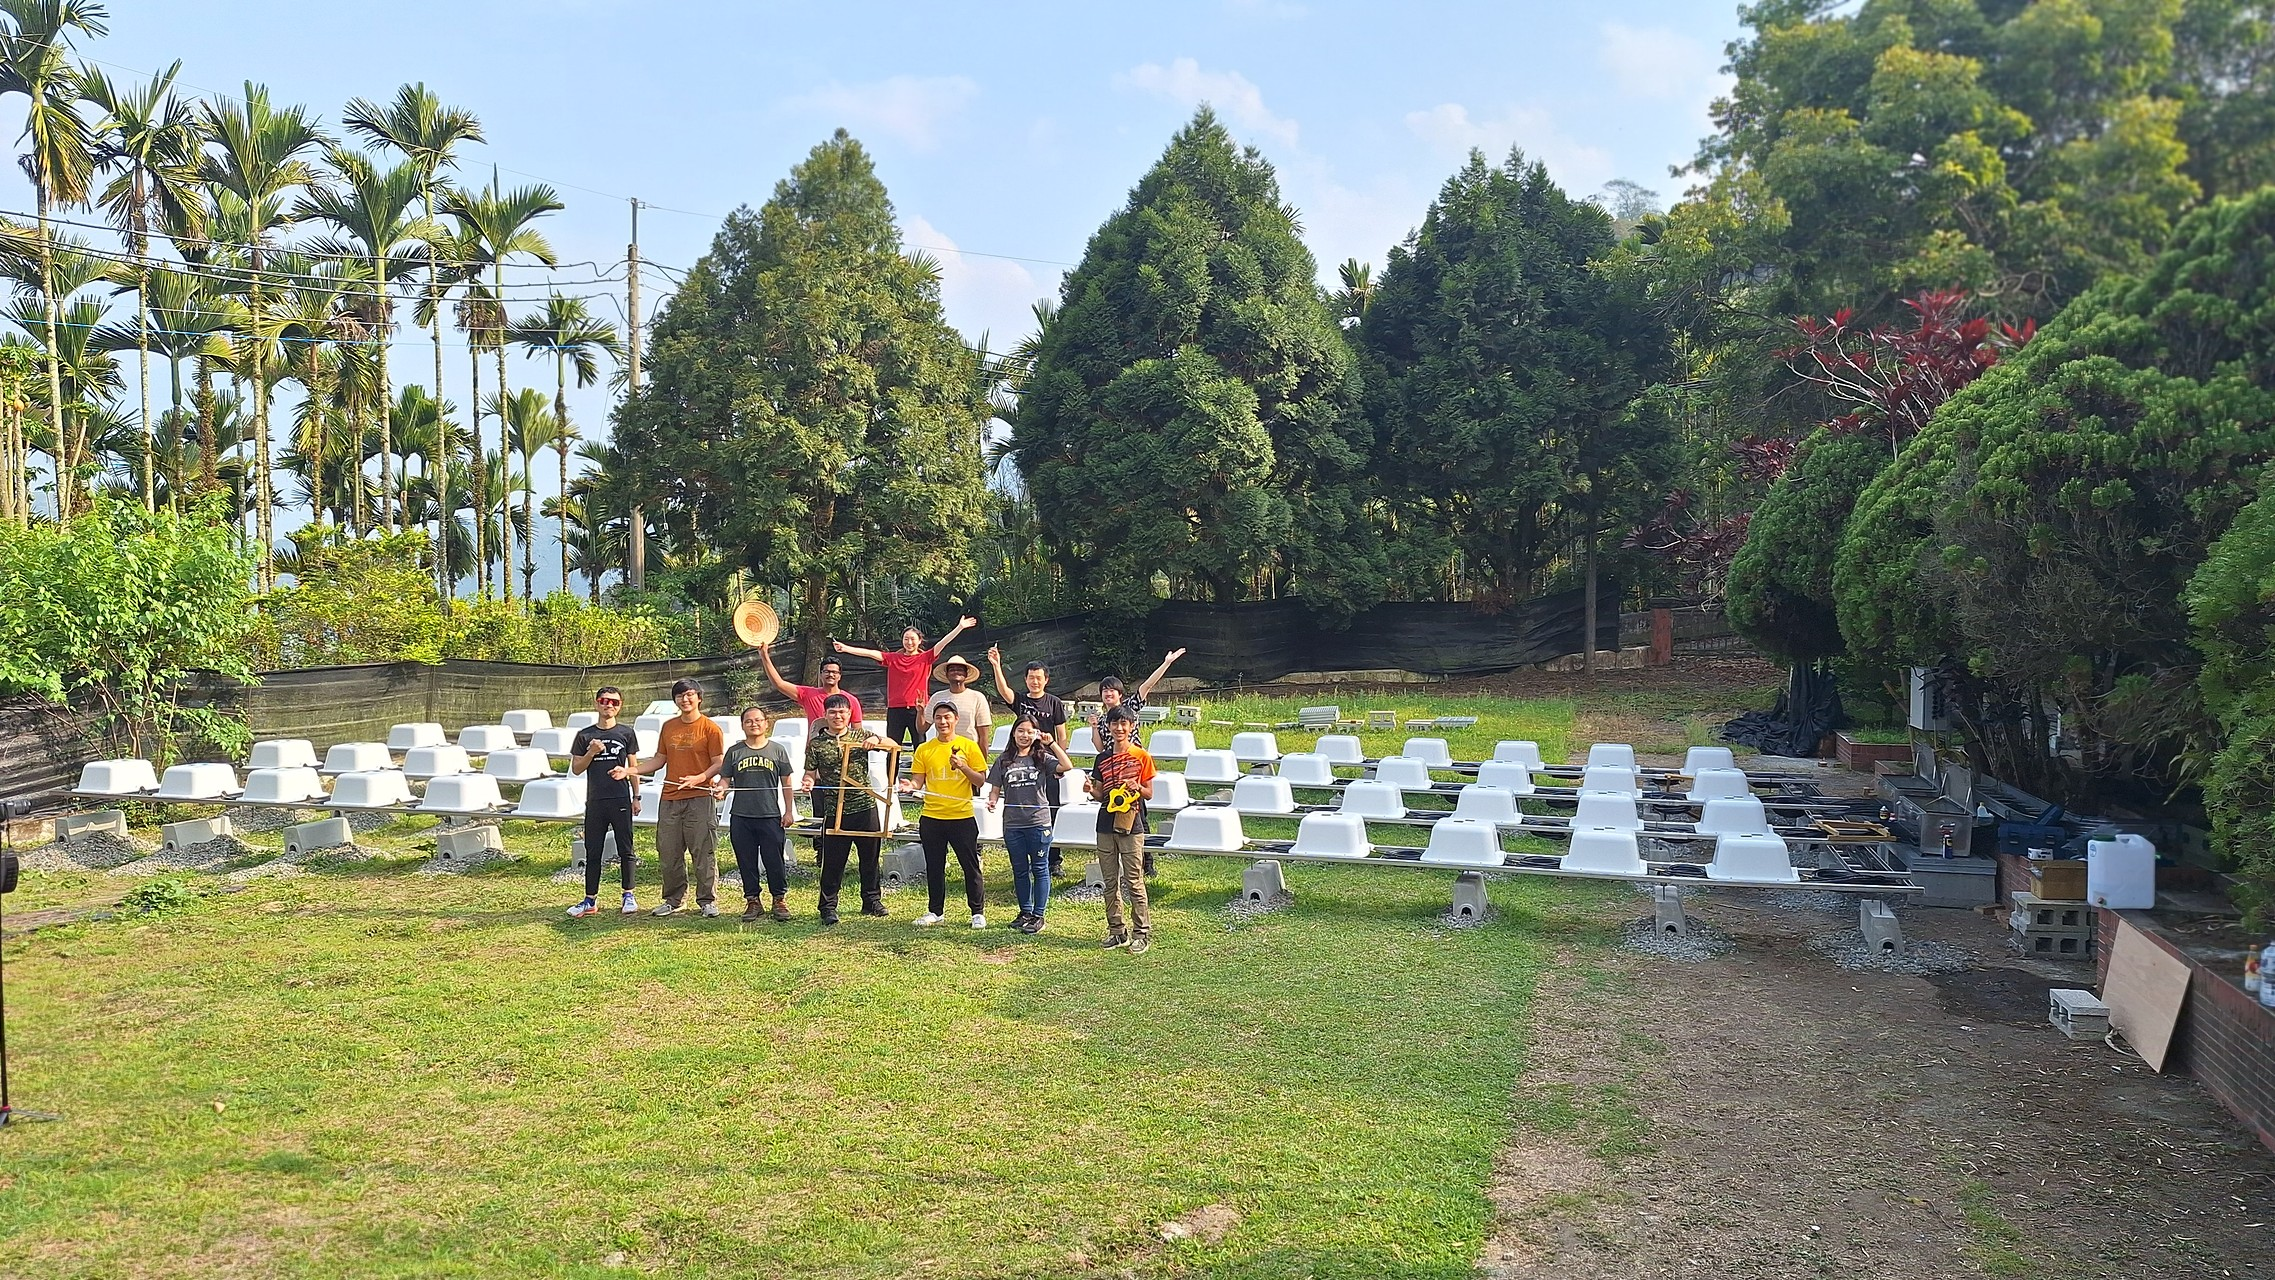
\includegraphics[width=4.5in]{Figures/nantou.JPEG}
  }


  \frame{
    \frametitle{Fugui}
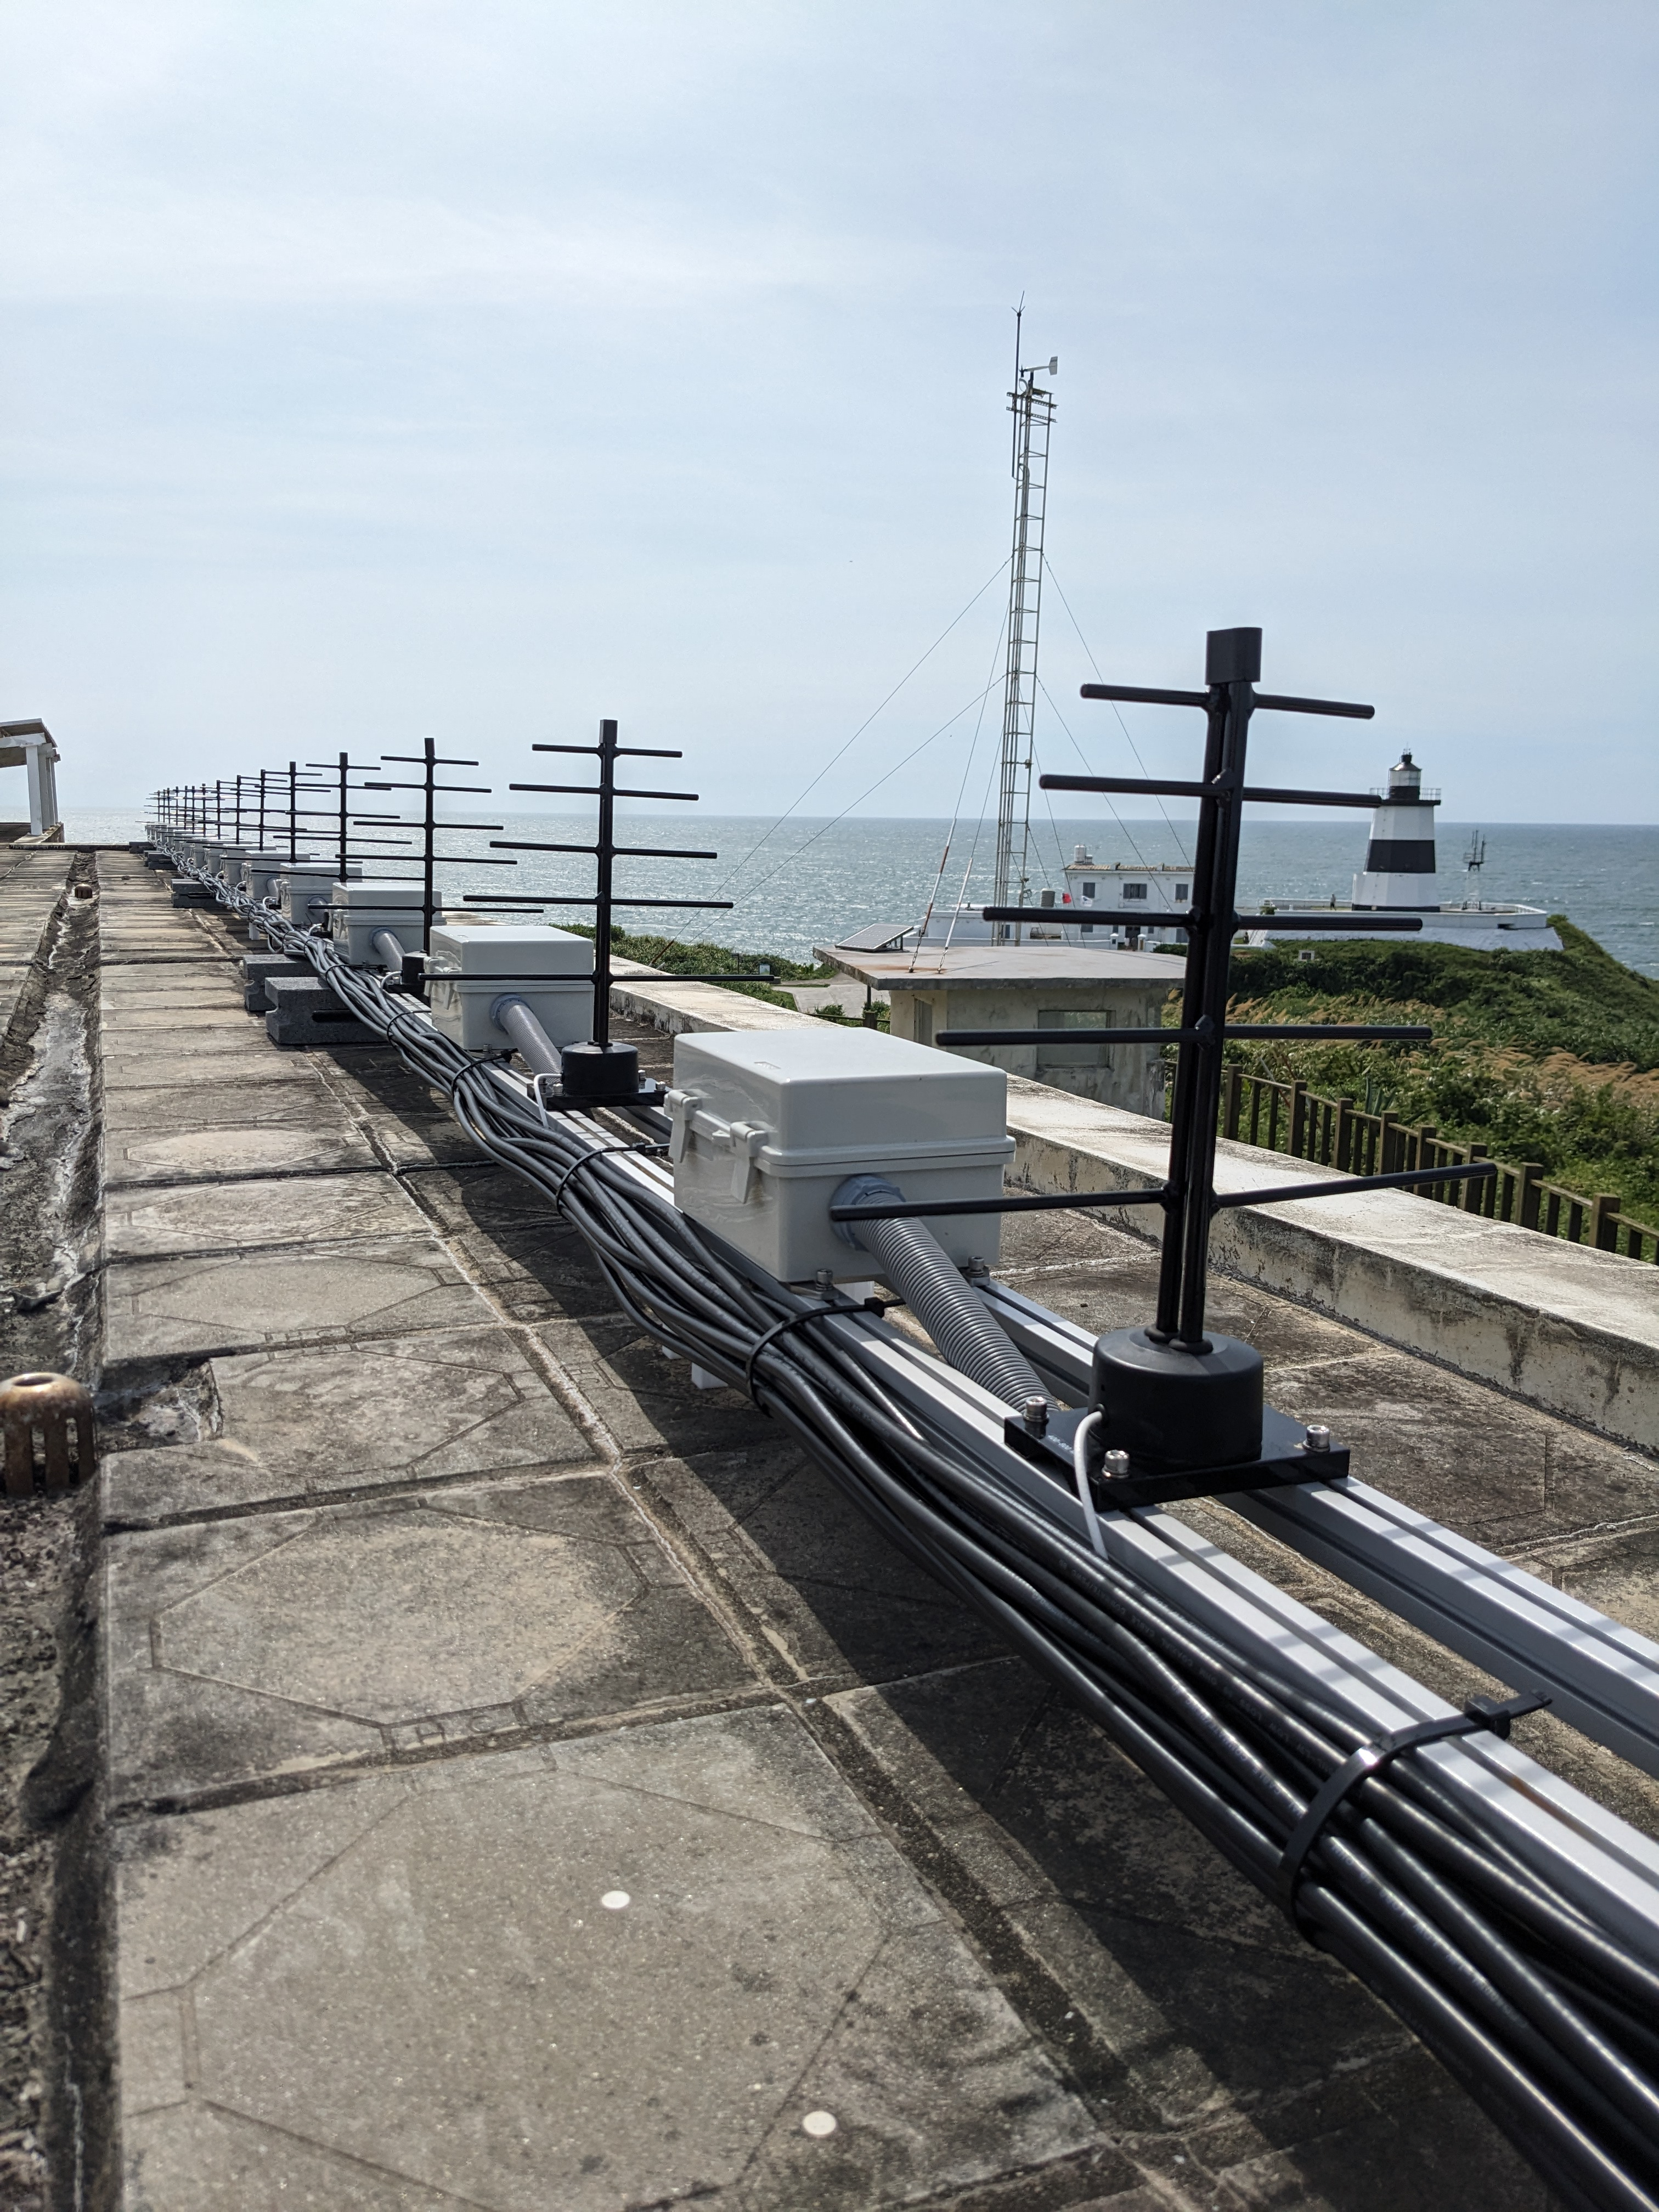
\includegraphics[width=2.5in]{Figures/bursttfugui.jpg}
  }

  \frame{
    \frametitle{VLBI}
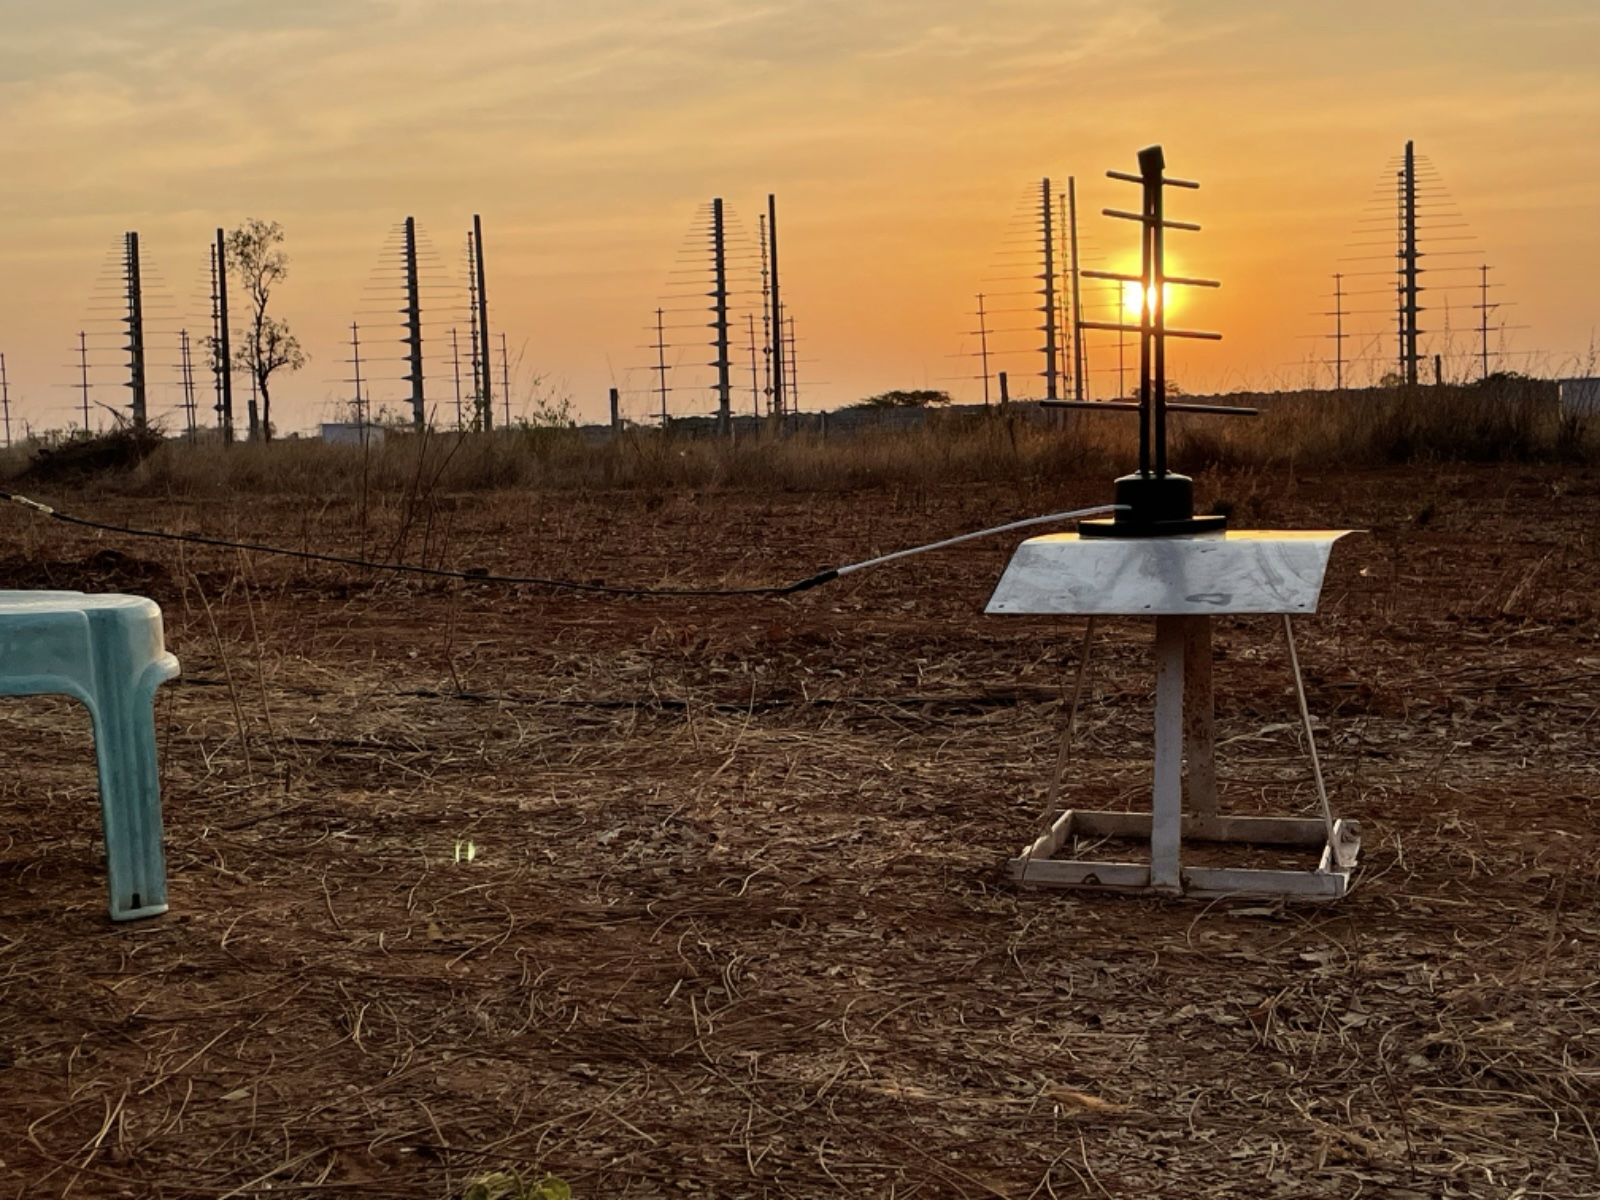
\includegraphics[width=1.95in]{Figures/gbd.jpg}
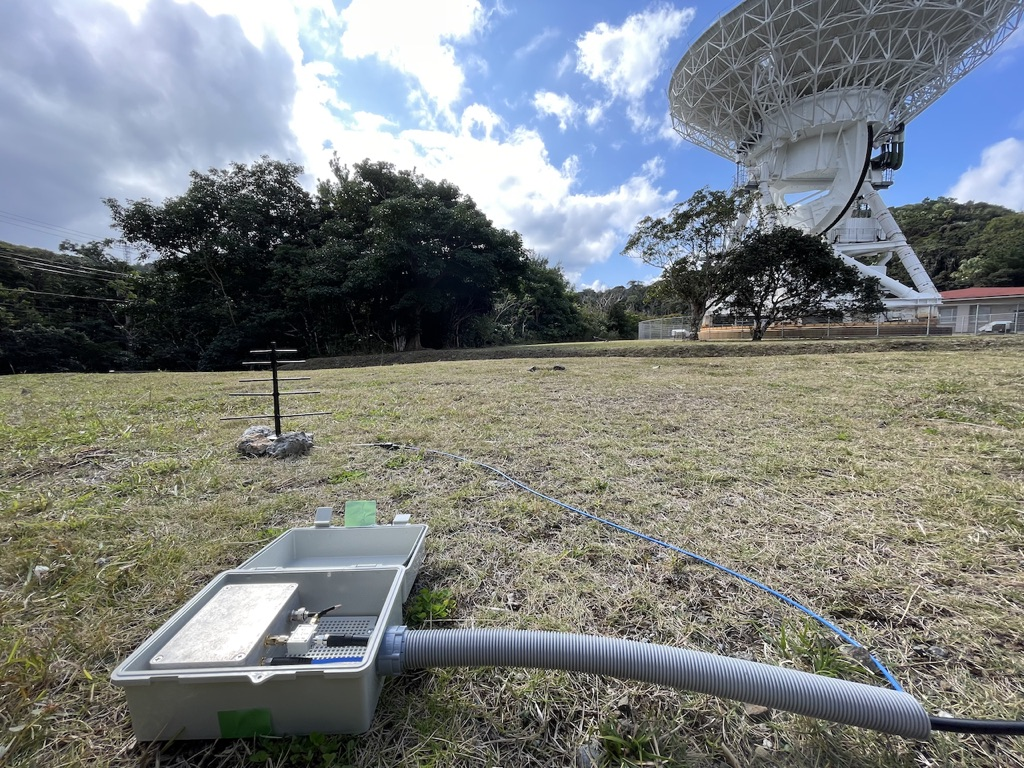
\includegraphics[width=1.95in]{Figures/ogasawara.jpeg}

\includegraphics[width=3.5in]{Figures/intlmap.png}
  }


  \frame{
%\vspace{-0.5in}
    \frametitle{Conclusions}
    \begin{itemize}
     \item wave optics changes nature of astrophysical observables: Coherent FRB/pulsar/GW      radiation one of the potentially most
      precise measurements in physics
      \item already makes microarcsecond images of pulsars
      \item ISM plasma screens modelled quantitatively as localized
        1-D features, no longer stochastic turbulent volume.
      \item next generation FRB telescopes for cosmic mass inventory,
        possibly dark energy/acceleration
      \item PTA weak diffractive lensing may give new tool for Hubble
        Constant tension
    \end{itemize}
  }

\end{document}
